\documentclass[
	11pt, 
	a4paper, 
	twoside,
	parskip=half*, % Line spacing for paragraphs
	openany, % Chapters can start on any page
	listof=totoc, % Include listings in the table of contents
	bibliography=totoc, % adding a bibliography to the table of contents
	index=totoc, % add index directory to the table of contents
  toc=chapterentrywithdots, % Set dots in the table of contents also for chapters
  numbers=noenddot, % removes the last dot after X.X.X.
  %chapterprefix=true % changes the display of the chapter, adds "Chapter" to the chapter number
]{scrbook}

\usepackage[utf8]{inputenc}
\usepackage{url}
\usepackage[T1]{fontenc}
\usepackage{pdfpages}
\usepackage{textcomp}
\usepackage{amsmath}

% ---------------------------
% |    Meta-Data for PDF    |
% ---------------------------
\usepackage[
  pdftex,
  pdfauthor={Nathan Rignall},
  pdftitle={Multi-Digit Classifier Report},
  pdfsubject={662086 - Machine Learning},
  pdfkeywords={ML}
  pdfproducer={LaTeX},
  pdfcreator={pdfLaTeX},
  pdfduplex={DuplexFlipLongEdge},
  pdflang={en},
  bookmarksopen,
  bookmarksnumbered,
]{hyperref}

% ------------------
% |    Settings    |
% ------------------
\usepackage[
    backend=biber, 
    style=authoryear-icomp, % alphabetic
    citestyle=authoryear-icomp, % alphabetic, authortitle
    date=short,
    % backref=true, % Display pages on which the reference is used
    maxnames=1, % affects the cites
    maxbibnames=3, % affects the bibliography
    pagetracker=true,
    isbn=false,    
    % block=ragged, % break urls
    % firstinits=true, % shorten first names
    backrefstyle=three+ % Combine pages
]{biblatex}

% Distance between bibliographical references
\setlength{\bibitemsep}{.5em}

% Indentation after the first line
\setlength{\bibhang}{2em}

% URL in the bibliography is in angle brackets
\DeclareFieldFormat{url}{<\url{#1}>}

% break too long urls
\setcounter{biburllcpenalty}{7000}
\setcounter{biburlucpenalty}{8000}

% Source of the bibliography file
\bibliography{sources/literature.bib}

% graphics
\usepackage{graphicx}
\graphicspath{ {images/} }
\DeclareGraphicsExtensions{.pdf,.png,.jpg,.jpeg,.gif}

% captions
\usepackage{caption}
\usepackage{subcaption}
% Table layout
\setlength{\tabcolsep}{0.5em} % for the horizontal padding
{\renewcommand{\arraystretch}{1.2} % for the vertical padding

% Table captions
\usepackage{caption} 
\captionsetup[table]{belowskip=12pt,aboveskip=4pt}
\usepackage{diagbox}

% Rotate tables
\usepackage{rotating}
\usepackage{varwidth}

% Footnotes with tables
\usepackage{footnote}
\makesavenoteenv{figure}

% Line breaks in table cells
\newcommand{\specialcell}[2][c]{%
  \begin{tabular}[#1]{@{}c@{}}#2\end{tabular}
}

% rotate content of table cell
\def\rot{\rotatebox} % usage: \rot{angle}{content}
% You can visit this website to find more color codes for LaTeX
% http://latexcolor.com/s

\usepackage{xcolor}

% colors
\definecolor{white}{rgb}{1,1,1}
\definecolor{black}{rgb}{0,0,0}
\definecolor{middlegray}{rgb}{0.5,0.5,0.5}
\definecolor{lightgray}{rgb}{.95,.95,.95}
\definecolor{arsenic}{rgb}{0.23, 0.27, 0.29}
\definecolor{arsenicLight}{rgb}{0.20, 0.20, 0.20}
\definecolor{darkgray}{rgb}{.4,.4,.4}
\definecolor{purple}{rgb}{0.65, 0.12, 0.82}
\definecolor{orange}{rgb}{0.8,0.3,0.3}
\definecolor{yac}{rgb}{0.6,0.6,0.1}
\definecolor{green}{rgb}{.2,0.6,0.3}
\definecolor{azure}{rgb}{0.0, 0.5, 1.0}
\definecolor{editorGray}{rgb}{0.95, 0.95, 0.95}
\definecolor{editorOcher}{rgb}{1, 0.5, 0}
\definecolor{editorGreen}{rgb}{0, 0.5, 0}
\definecolor{orange}{rgb}{1,0.45,0.13}		
\definecolor{olive}{rgb}{0.17,0.59,0.20}
\definecolor{brown}{rgb}{0.69,0.31,0.31}
\definecolor{purple}{rgb}{0.38,0.18,0.81}
\definecolor{lightblue}{rgb}{0.1,0.57,0.7}
\definecolor{lightred}{rgb}{1,0.4,0.5}

\definecolor{vscodered}{HTML}{E53935}
\definecolor{vscodelightred}{HTML}{EF5350}
\definecolor{vscodeblue}{HTML}{1565C0}
\definecolor{vscodegreen}{HTML}{66BB6A}

\definecolor{lightblack}{HTML}{212121}
\definecolor{darkraspberry}{rgb}{0.53, 0.15, 0.34}

% blue hues
\definecolor{bleudefrance}{rgb}{0.19, 0.55, 0.91}
\definecolor{brandeisblue}{rgb}{0.0, 0.44, 1.0}
\definecolor{blue(ncs)}{rgb}{0.0, 0.53, 0.74}
\definecolor{coolblack}{rgb}{0.0, 0.18, 0.39}

% red hues
\definecolor{coralred}{rgb}{1.0, 0.25, 0.25}
\definecolor{darkred}{rgb}{0.55, 0.0, 0.0}

% geometry
\usepackage{geometry}
\geometry{left=25mm, right=25mm, top=25mm, bottom=30mm}

\usepackage[automark]{scrlayer-scrpage}
\pagestyle{scrheadings}
\automark*[section]{}
\ohead{\headmark} % name of the current section
\ihead{}
\ofoot{\thepage} % page number

% footnote gap
\addtolength{\skip\footins}{1ex}
\addtolength{\footnotesep}{0.5ex}

% prevent footnote page break
\interfootnotelinepenalty=10000

% prevent page break in the middle of a paragraph
\widowpenalties 1 10000

% line spacing
\usepackage[onehalfspacing]{setspace}

% text does not have to go to the end of a page
\raggedbottom

% space before and after chapter headings
\RedeclareSectionCommand[beforeskip=0pt,afterskip=.6cm,font=\fontsize{18}{20}\selectfont]{chapter}
% \RedeclareSectionCommand[beforeskip=10pt,afterskip=.3cm,font=\fontsize{18}{25}\selectfont]{section}
% \RedeclareSectionCommand[beforeskip=10pt,afterskip=.3cm,font=\fontsize{16}{25}\selectfont]{subsection}
% \RedeclareSectionCommand[beforeskip=0pt,afterskip=.3cm,font=\fontsize{14}{25}\selectfont]{subsubsection}

\usepackage{mwe}

% chapter style
\renewcommand*{\chapterformat}{%
  \thechapter\enskip
  \textcolor{gray!70}{\rule[-\dp\strutbox]{1pt}{\baselineskip}}\enskip
}
\setkomafont{disposition}{\normalcolor\bfseries}

% adjust paragraphs
%\addtokomafont{paragraph}{\itshape}
%\setkomafont{subsubsection}{\large}
%\setkomafont{paragraph}{\normalsize\itshape}
\setkomafont{paragraph}{\normalsize}

% % layout of the paragraphs
% % paragraphs look like the subsubsections
% \RedeclareSectionCommands[
%     beforeskip=-3.25ex plus -1ex minus -0.2ex,
%     afterskip=1sp, % smallest possible positive value
% ]{paragraph,subparagraph}

% Bold caption labels
\setkomafont{captionlabel}{\normalsize\bfseries} 
% \usepackage[font=sf]{caption} % Captions without serifs
% for the links in toc
\usepackage{hyperref}
\hypersetup{
    colorlinks,
    citecolor=black,
    filecolor=black,
    linkcolor=black,
    urlcolor=black,
    pdfstartview= % fit zoom size to the viewer
}
%\newcommand{\code}[1]{\colorbox{lightgray}{\texttt{#1}}}
%\lstinline{snippet}
%http://tex.stackexchange.com/questions/65291/code-snippet-in-text

% This "\code{my code}" can be used to highlight small code snippets in the text like names of variables or methods.
\newcommand{\code}[1]{\textcolor{black}{\texttt{#1}}}

% The "\todo{this still has to be done}" is a command that highlights todos in the text.
\newcommand{\todo}[1]{\textcolor{vscodered}{TODO: \texttt{#1}}}
% Adding package bookmark improves bookmarks handling.
% More features and faster updated bookmarks.
\usepackage{bookmark}

% \pdfbookmark[<level>]{<title>}{<dest>}

% toc is part of the bookmarks but not part the toc itself
% \pdfbookmark[section]{\contentsname}{toc}


\begin{document}

% -------------------
% |    Titlepage    |
% -------------------
\titlehead{\centering University of Hull}
\subject{662086 - Machine Learning}
\title{Multi-Digit Classifier Report}
\author{Nathan Rignall}
\date{\today}
\maketitle

% ---------------------------
% |    Table of contents    |
% ---------------------------
\pdfbookmark[section]{\contentsname}{toc}
\newpage\thispagestyle{empty}
{
  \pagestyle{empty}
  \addtocontents{toc}{\protect\thispagestyle{empty}} 
  \tableofcontents
  \clearpage
}

% -----------------
% |    Indexes    |
% -----------------
\frontmatter
\pagenumbering{arabic}
\listoffigures
\listoftables

% ------------------
% |    Chapters    |
% ------------------
\mainmatter
\setcounter{page}{1}
\chapter{Visualisation}
This report outlines the steps taken to develop a handwritten multi-digit classifier using multiple machine learning techniques. A random sample of images and labels from the provided dataset displays the challenges of implementing such classifier. The red markings in \autoref{fig:sampleImage} highlight a few poorly written digits and additional noise.

\begin{figure}[h]
    \centering
    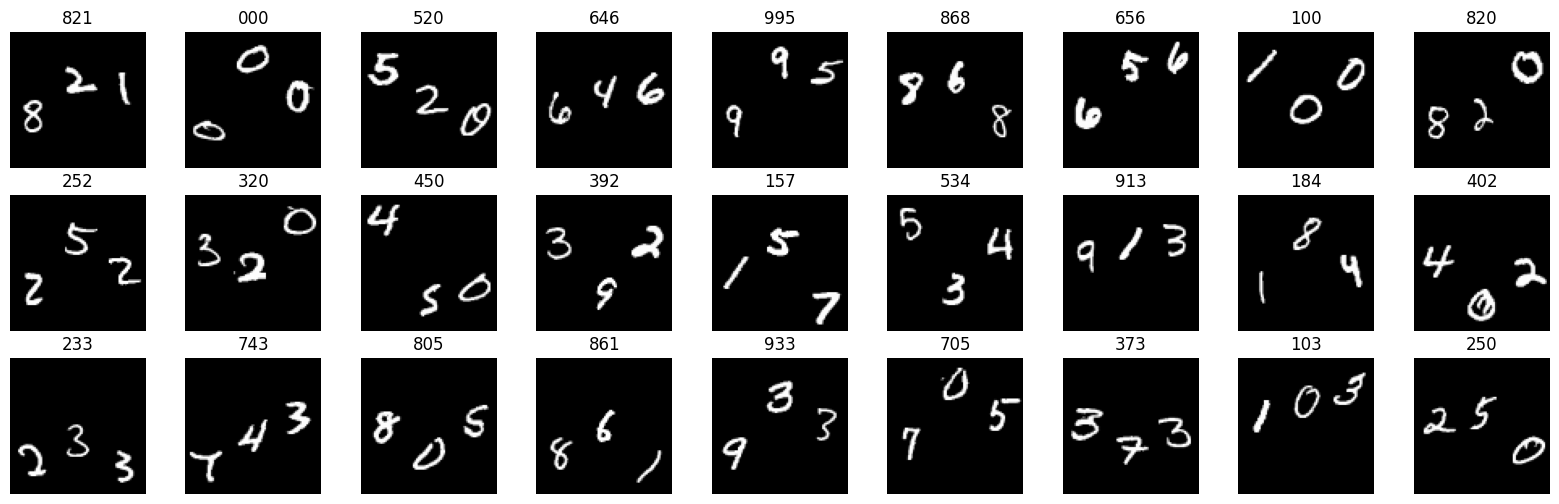
\includegraphics[width=\textwidth, height=\textheight,keepaspectratio]{task1/digitSample}
    \caption[Random sample of images and labels]
    {Random sample of images and labels}
    \label{fig:sampleImage}
\end{figure}

There are 640, 200 and 160 classes present in the train, test, and validation sets, all classes contain 100 images.  The images are greyscale. The distribution graphs display when a class is present in a set. The red lines indicate which classes are present in the test or validation sets but not present in the train set. Unfortunately, this shows that all classes in the test and validation set are not in the train set. Using the dataset as it is, with single labels, learning from the training set cannot transfer into the validation and test sets.

\begin{figure}[h]
    \centering
    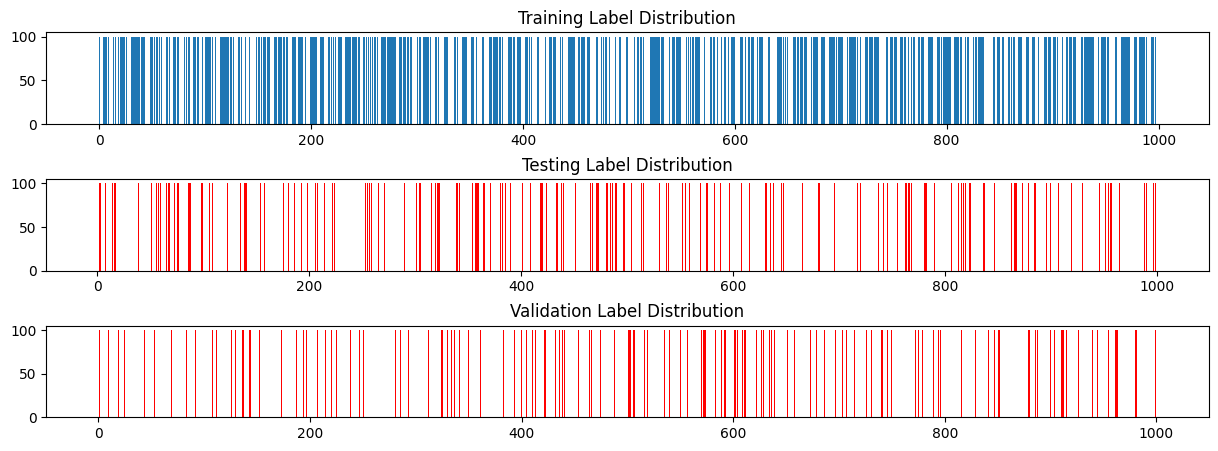
\includegraphics[width=\textwidth, height=\textheight,keepaspectratio]{task1/classDistribution}
    \caption[Distribution graph for datasets]
    {Distribution graph for test/train/validation datasets}
    \label{fig:classDistribution}
\end{figure}

Instead, this should be treated as a multi-label classification problem, with each label representing a digit. For example, the image containing 123 does not contain a single label of “123” but rather three labels of “1”, “2”, and “3”.

When treated as a multi-label classification problem, analysis of the placement of the digits can take place. The heatmap displays the proportion of the digits at a specific location within the images. Ideally the distribution is 0.1 per digit (10\%) at each location. Train is the most evenly distributed set in \autoref{fig:heatmap}, likely due to its size.  This is most optimal as during training the model shall receive an even exposure of all digits.

\begin{figure}[h]
    \centering
    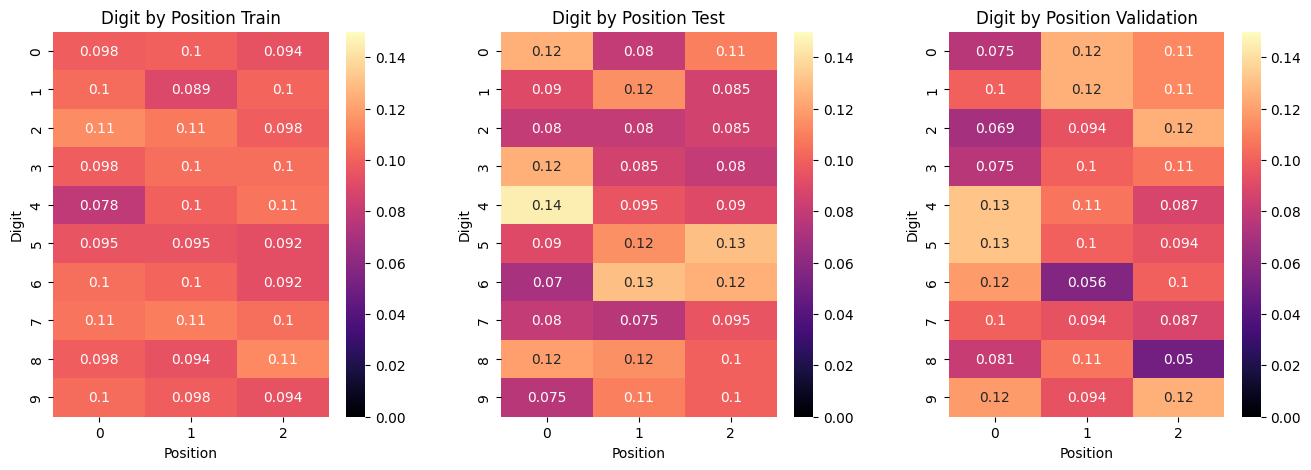
\includegraphics[width=\textwidth, height=5cm,keepaspectratio]{task1/classHeatmap}
    \caption[Heatmap for class distribution in dataset]
    {Heatmap for class distribution in dataset}
    \label{fig:heatmap}
\end{figure}

\begin{figure}[h]
    \centering
    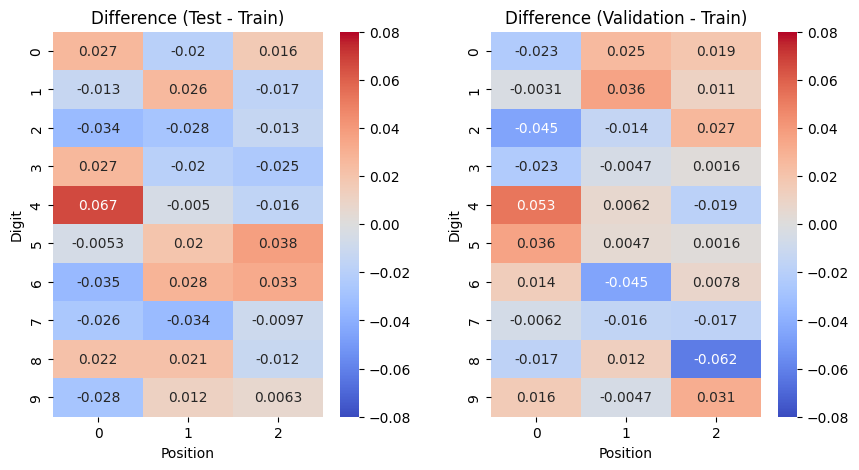
\includegraphics[width=\textwidth, height=5cm,keepaspectratio]{task1/classDifferenceHeatmap}
    \caption[Heatmap for difference in class distribution across dataset]
    {Heatmap for difference in class distribution across dataset}
    \label{fig:digitHeatmap}
\end{figure}

The additional heatmaps in \autoref{fig:digitHeatmap} display the difference between the test and validation sets against the train datasets, designed to highlight any gaps in training. Any digits marked with a positive difference (marked with a red shade) may perform worse in the validation and training evaluations. Digit four in position 1 appears to contain the most positive difference relative to the training set.
\chapter{Training}

\section{Single Model Training}
To set a baseline we can treat this as a simple classification problem with one thousand possible classes. With a complete dataset this could perform moderately well. However, as all classes in the validation and test sets are not present in the train, it can be expected the models will achieve an accuracy of near zero. Assuming accuracy is measured using the total number of labels entirely classified as correct, rather than individual digits.

\subsection{Convolutional Neural Network}
To form the basis of our multi-digit classifier we shall use an existing convolutional neural network (CNN) architecture with slight modifications. \autocite{biswasEfficientCNNModel2021} conducted a survey into optimal network architectures, the most optimal performed at an accuracy of 99.53\%. \autoref{fig:cnnArchitecture} displays such layer design in combination with additional dropout layers in between the fully connected layers. Dropout layers, a regularization method, are a simple yet affective way to reduce the likelihood of overfitting \autocite{srivastavaDropoutSimpleWay2014}. This model contains a six-layer CNN plus a two-layer dense classifier.

\begin{figure}[!htbp]
    \centering
    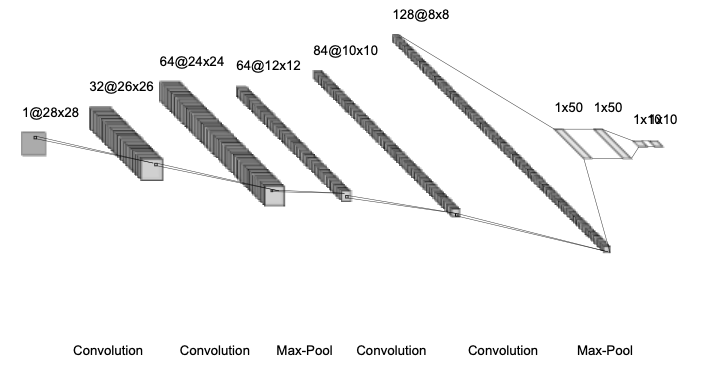
\includegraphics[width=\textwidth, height=\textheight,keepaspectratio]{task2/cnnArchitecture}
    \caption[Convolutional Neural Network Architecture]
    {CNN architecture generated using Alex Lenail}
    \label{fig:cnnArchitecture}
\end{figure}

\pagebreak

Using the Adam optimiser with a learning rate of 0.001 and the categorical crossentropy loss function an accuracy of 0.0\% is achieved on the test set.  

The learning graphs in \autoref{fig:cnnLearning} could suggest the model is overfitting, when a model performs well on the training data but does not generalize well \autocite{geronHandsOnMachineLearning2019}. However, this is because all test and validation classes are missing in the test set, likely not due to the model being too complex. No amount of regularization could improve this model's performance. 

\begin{figure}[!htbp]
    \centering
    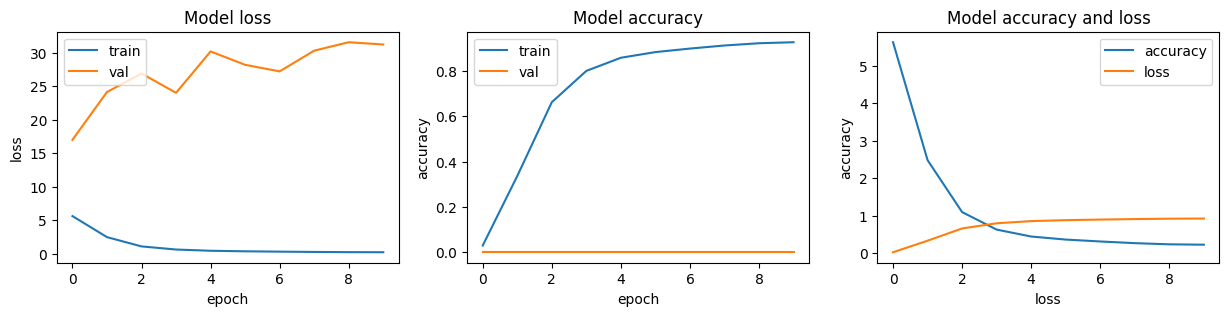
\includegraphics[width=\textwidth, height=\textheight,keepaspectratio]{task2/cnnLearningGraph}
    \caption[Learning graphs for CNN]
    {Learning graphs for CNN}
    \label{fig:cnnLearning}
\end{figure}

This theory is further reenforced in \autoref{fig:cnnPredictions} whereby the predictions are mostly correct on unseen data. Approximately two digits within the predictions are true versus the labels, but never three. Missing data is the cause of these false predictions.

\begin{figure}[!htbp]
    \centering
    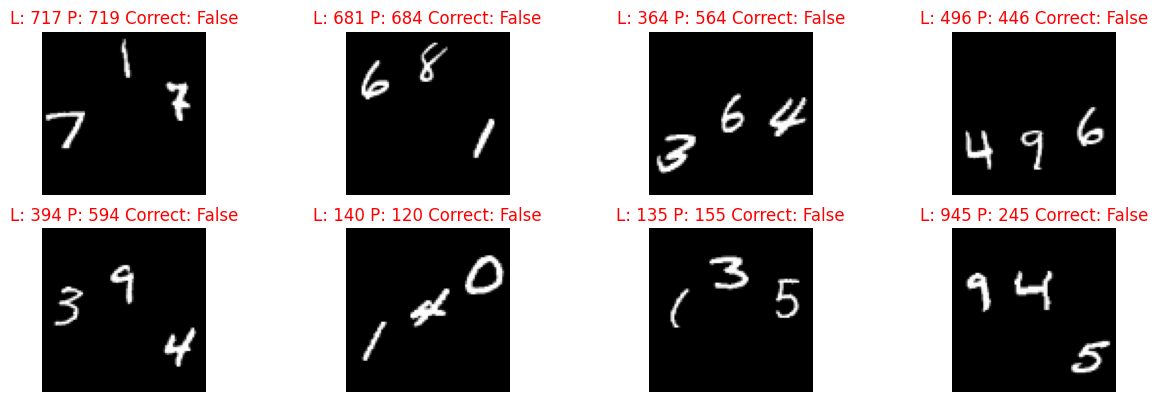
\includegraphics[width=\textwidth, height=\textheight,keepaspectratio]{task2/cnnPredictions}
    \caption[Predictions for CNN]
    {Predictions for CNN}
    \label{fig:cnnPredictions}
\end{figure}

In the model's current state, it is impossible to complete hyperparameter tuning as the accuracy metric on both the validation and test sets is zero. No hyperparameter tuner could deduce what parameters are better if the difference in accuracy is negligible. In order to conduct tuning, a new performance metric must be used if the overall model architecture is not changed. Currently accuracy is evaluated using an exact comparison between two labels. For instance, the label “717” is not equivalent to “719” however, this is technically 66.66\% correct. If the accuracy is measured on a per-digit basis we can hope that the validation accuracy improves so that tuning can occur.

The original dataset shall not be modified to remove this poor distribution as it mirrors a real-world problem scenario where not all classes are present.

Using the hyperparameter values displayed in \autoref{tbl:hyperCNN} an accuracy of 66.56\% is achieved on the test set using the per-digit metric. This value is exactly as expected as the classifier is able to successfully classify approximately two thirds of the digits. This proves the model is not overfitting from an overly complex model, rather the classification layer is simply missing entire classes. Unfortunately using the traditional per-class metric, an accuracy of 0.0\% is observed.

\bgroup
    \begin{table}[!htbp]
        \centering
        \begin{tabular}{ll|c}
            \hline
            Parameter & Values & Selected \\ \hline
            kernel\_size\_1 & 2, 3, 4, 5 & 4 \\
            kernel\_size\_2 & 2, 3, 4, 5 & 3 \\
            kernel\_size\_3 & 2, 3, 4, 5 & 4 \\
            kernel\_size\_4 & 2, 3, 4, 5 & 4 \\
            pool\_size\_1 & 2, 3, 4 & 4 \\
            pool\_siz\_2 & 2, 3, 4 & 3 \\
            dropout\_1 & 0.2, 0.8, step=0.1 & 0.6 \\
            dropout\_2 & 0.2, 0.8, step=0.1 & 0.5 \\
            dense\_layer\_units & 1000, 2000, 3000, 4000, 5000 & 3000 \\
            learning\_rate & min=0.0001, max=0.1, sampling="LOG" & 0.00024 \\
        \end{tabular}
        \caption{Hyperparameter values for CNN}
        \label{tbl:hyperCNN}
    \end{table}
\egroup

The learning graph in \autoref{fig:cnnHyperLearning}, containing the unmodified loss metric, is almost identical to that of the loss graph in \autoref{fig:cnnHyperConfusionMatrix}. This is because the model's architecture hasn't fundamentally changed. The accuracy graph does reflect the new score, but the overall performance is similar to the unoptimized model. The underlying convolutional and pooling layers are likely correct, but the dense layers are lacking the exposure from the additional classes.

\begin{figure}[!htbp]
    \centering
    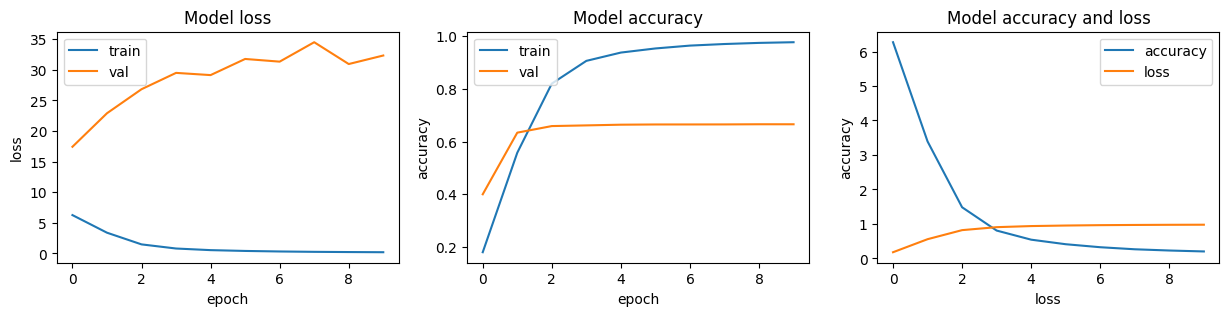
\includegraphics[width=\textwidth, height=\textheight,keepaspectratio]{task2/cnnHyperLearningGraph}
    \caption[Learning graphs for hyperparameter tuned CNN]
    {Learning graphs for hyperparameter tuned CNN}
    \label{fig:cnnHyperLearning}
\end{figure}

% \begin{figure}[!htbp]
%     \centering
%     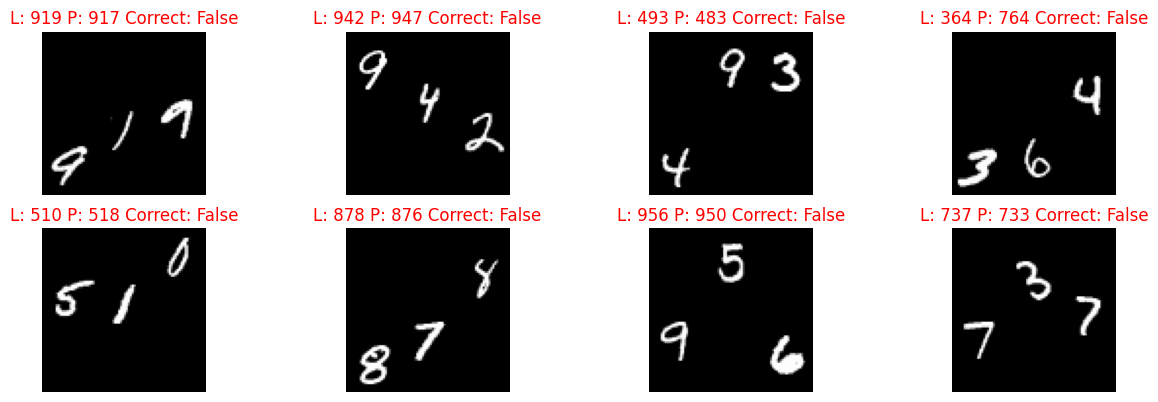
\includegraphics[width=\textwidth, height=\textheight,keepaspectratio]{task2/cnnHyperPredictions}
%     \caption[Predictions for hyperparameter tuned CNN]
%     {Predictions for hyperparameter tuned CNN}
%     \label{fig:cnnHyperPredictions}
% \end{figure}

\begin{figure}[!htbp]
    \centering
    \begin{subfigure}{0.3\textwidth}
        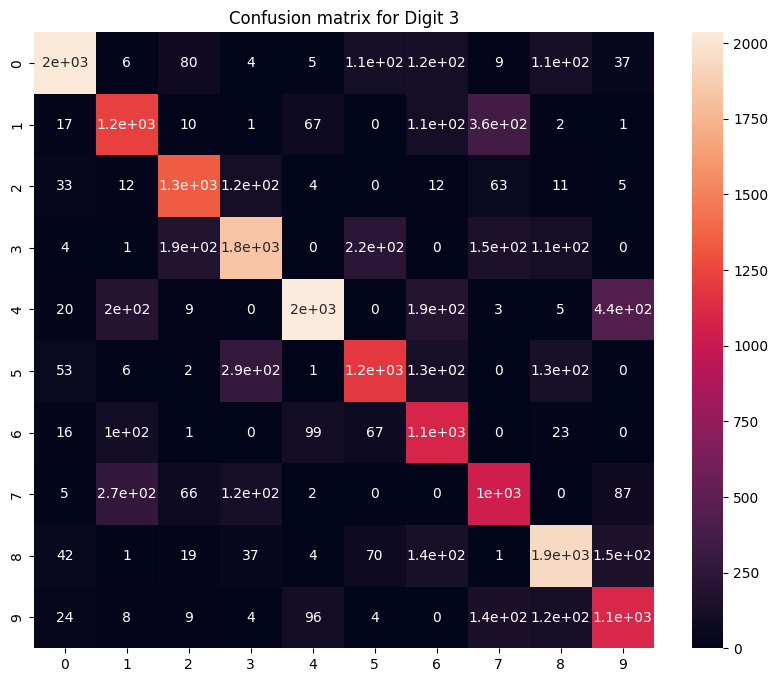
\includegraphics[width=\textwidth]{task2/cnnHyperConfusion/digit1}
        \caption{Digit 1}
        \label{fig:cnnHyperConfusionMatrix1}
    \end{subfigure}
    \begin{subfigure}{0.3\textwidth}
        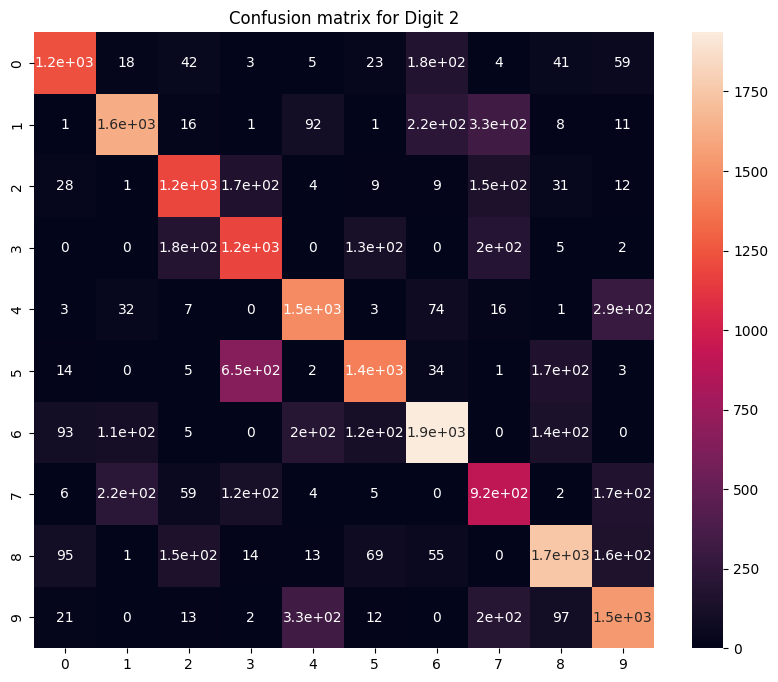
\includegraphics[width=\textwidth]{task2/cnnHyperConfusion/digit2}
        \caption{Digit 2}
        \label{fig:cnnHyperConfusionMatrix2}
    \end{subfigure}
    \begin{subfigure}{0.3\textwidth}
        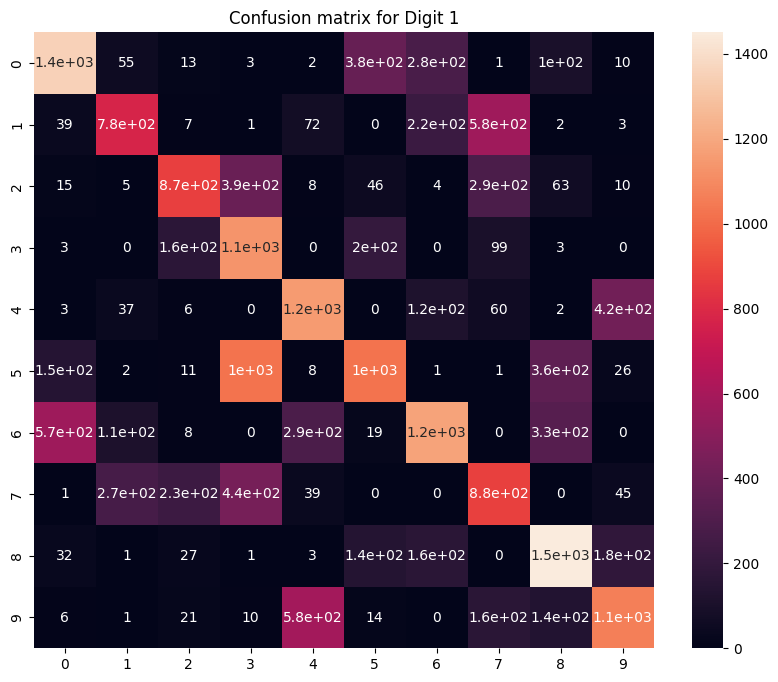
\includegraphics[width=\textwidth]{task2/cnnHyperConfusion/digit3}
        \caption{Digit 3}
        \label{fig:cnnHyperConfusionMatrix3}
    \end{subfigure}
    \caption{Confusion matrices for hyperparameter tuned CNN}
    \label{fig:cnnHyperConfusionMatrix}
\end{figure}

\pagebreak
\subsection{Convolutional Neural Network with Custom Encode}
Without making any improvements to the model itself we can attempt to improve its accuracy on unseen classes by changing how the classes are encoded.

Currently the labels are one-hot encoded. As there are a thousand classes, this produces an array of size 1000. Learning from individual digits cannot transfer across the classifier. As far as the neural network is concerned, there is no similarity between 312 and 345, despite the digit three being repeated across the two classes. This is one of the reasons why the test set performs so poorly.

If instead the digits are encoded in such a way so that learning can be transferred across classes, the model performance could be improved. One possible technique is one-hot encoding each digit individually and concatenating the result. This produces three arrays of size ten that are concatenated together to produce an array of size thirty, \autoref{fig:oneHotEncoding} versus \autoref{fig:customOneHotEncoding}. The output space is no longer significantly expanded to one thousand and is instead thirty. Now training does not require all one thousand classes to be present, instead each digit location must just include a class from one to ten.

\begin{figure}[!htbp]
    \centering
    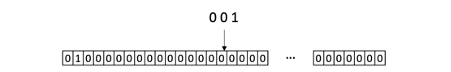
\includegraphics[width=\textwidth, height=\textheight,keepaspectratio]{task2/labelEncodingTraditional}
    \caption[Traditional one-hot encoding method for classification]
    {Traditional one-hot encoding method for classification}
    \label{fig:oneHotEncoding}
\end{figure}

\begin{figure}[!htbp]
    \centering
    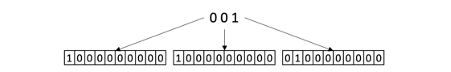
\includegraphics[width=\textwidth, height=\textheight,keepaspectratio]{task2/labelEncodingCustom}
    \caption[Custom one-hot encoding method for classification]
    {Custom one-hot encoding method for classification}
    \label{fig:customOneHotEncoding}
\end{figure}

In order for the model to understand this method of encoding, a custom loss function and accuracy metric must be created. For the loss function, we can use the categorical crossentropy loss function for each digit by slicing the input arrays and summing the loss. The custom accuracy metric can use the same technique of slicing but instead use the categorical accuracy metric and average. A per-digit accuracy of 98.12\% is realised on the test set after ten epochs of training.

\begin{figure}[!htbp]
    \centering
    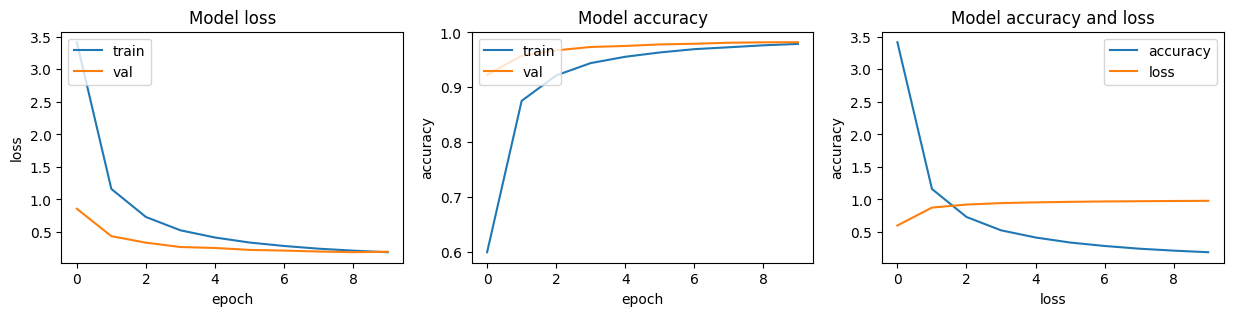
\includegraphics[width=\textwidth, height=\textheight,keepaspectratio]{task2/cnnModLearningGraph}
    \caption[Learning graphs for CNN with custom encoding]
    {Learning graphs for CNN with custom encoding}
    \label{fig:cnnCustomLearning}
\end{figure}

The learning graphs display the model is not overfitting, the validation set outperforms the training set. This is most likely due to the validation set being of a higher quality and smaller sample size than the training.

\begin{figure}[!htbp]
    \centering
    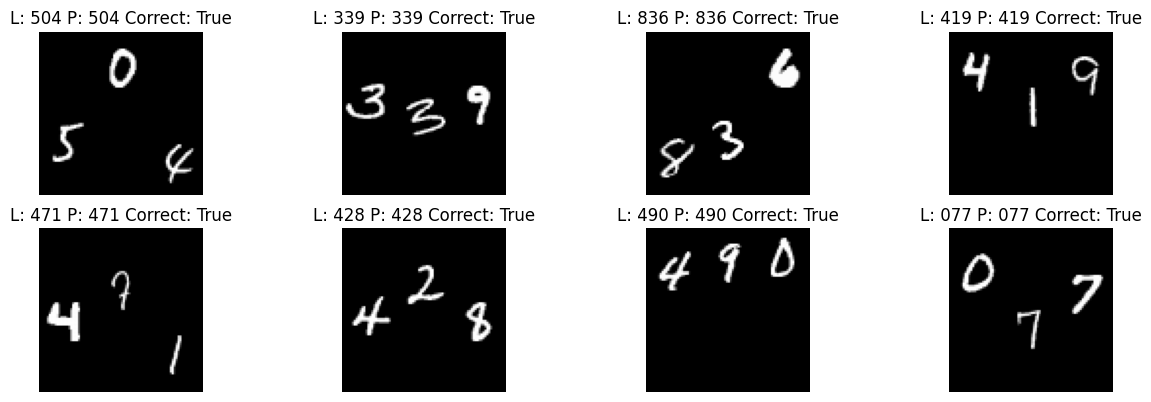
\includegraphics[width=\textwidth, height=\textheight,keepaspectratio]{task2/cnnModPredictions}
    \caption[Predictions for CNN with custom encoding]
    {Predictions for CNN with custom encoding}
    \label{fig:cnnCustomPredictions}
\end{figure}

The random sample of images in \autoref{fig:cnnCustomPredictions} shows that the model is performing well but some challenging digits are still being miss-classified.

The model is also fairly balanced, no digit location or class is performing significantly worse than another. The even distribution of accuracy and F1 scores in \autoref{fig:cnnModConfusionMatrix} and balanced confusion matrices in \autoref{tbl:accuracyCNNMod} reenforce this.

\begin{figure}[!htbp]
    \centering
    \begin{subfigure}{0.3\textwidth}
        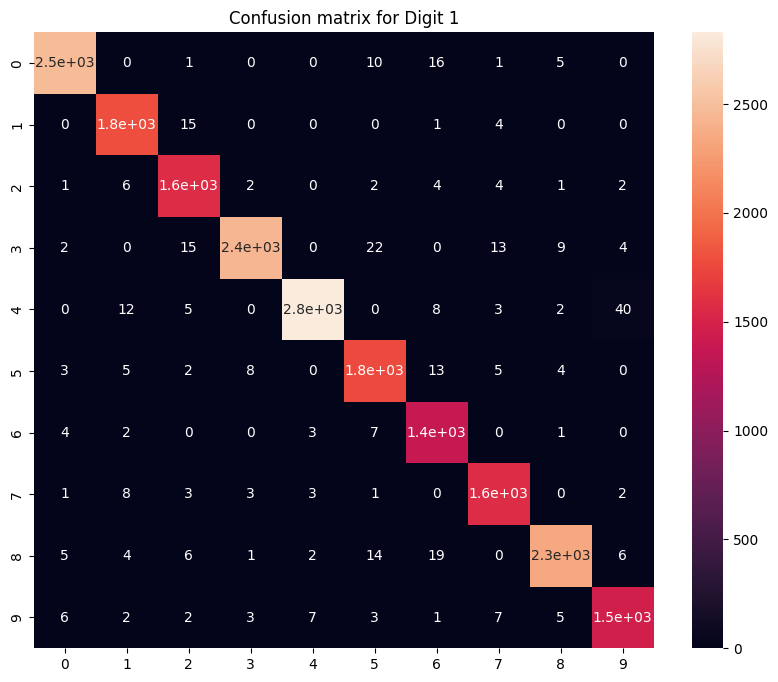
\includegraphics[width=\textwidth]{task2/cnnModConfusion/digit1}
        \caption{Digit 1}
        \label{fig:cnnModConfusionMatrix1}
    \end{subfigure}
    \begin{subfigure}{0.3\textwidth}
        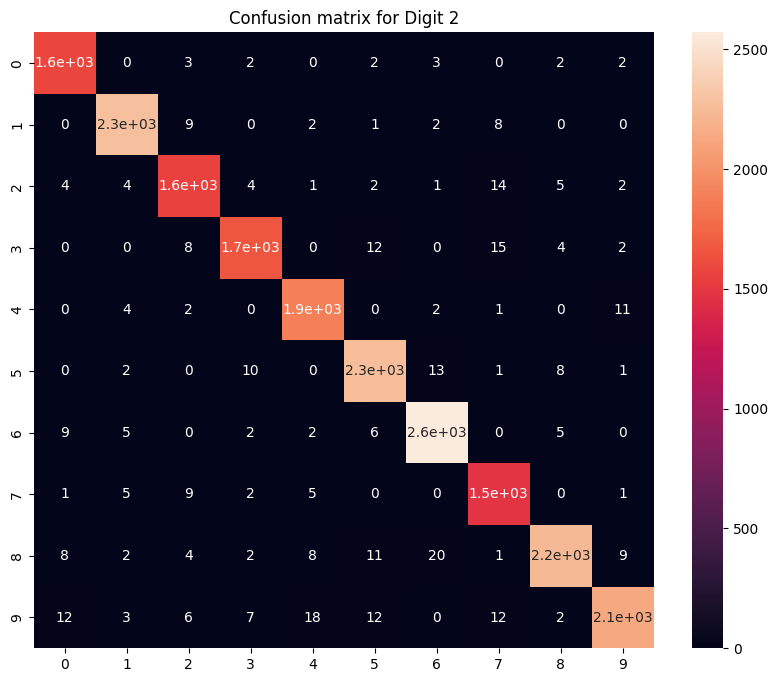
\includegraphics[width=\textwidth]{task2/cnnModConfusion/digit2}
        \caption{Digit 2}
        \label{fig:cnnModConfusionMatrix2}
    \end{subfigure}
    \begin{subfigure}{0.3\textwidth}
        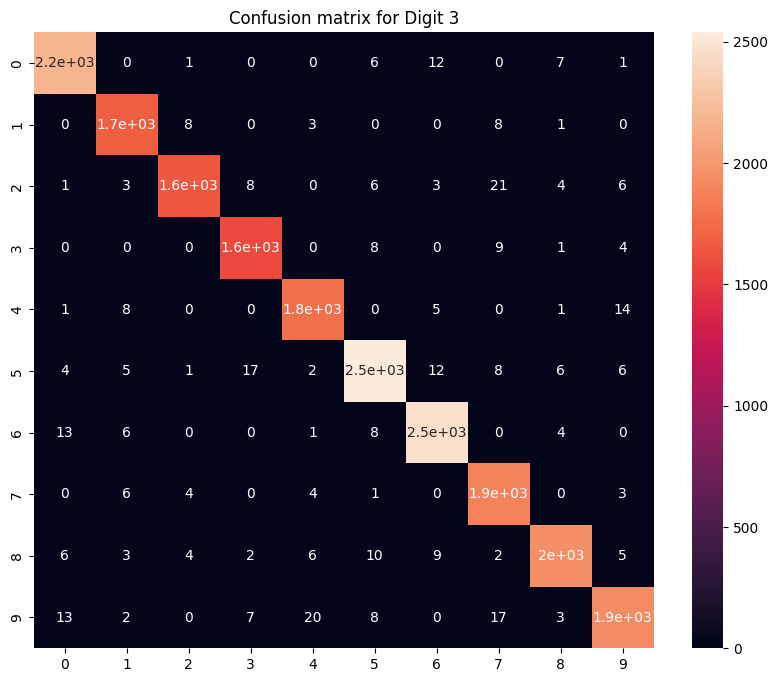
\includegraphics[width=\textwidth]{task2/cnnModConfusion/digit3}
        \caption{Digit 3}
        \label{fig:cnnModConfusionMatrix3}
    \end{subfigure}
    \caption{Confusion matrices for CNN with custom encoding}
    \label{fig:cnnModConfusionMatrix}
\end{figure}

\bgroup
    \begin{table}[!htbp]
        \centering
        \begin{tabular}{l|cc}
            \hline
            & Accuracy & F1 Score \\ \hline
            Digit 1 & 0.9810 & 0.9798 \\
            Digit 2 & 0.9821 & 0.9817 \\ 
            Digit 3 & 0.9811 & 0.9810 \\
        \end{tabular}
        \caption{Accuracy and F1 scores for CNN with custom encoding}
        \label{tbl:accuracyCNNMod}
    \end{table}
\egroup

Using the validation set the model can undergo hyperparameter tuning. The dense layer is reduced to resemble the output layer more closely.

\bgroup
    \begin{table}[!htbp]
        \centering
        \begin{tabular}{ll|c}
            \hline
            Parameter & Values & Selected \\ \hline
            kernel\_size\_1 & 2, 3, 4, 5 & 2 \\
            kernel\_size\_2 & 2, 3, 4, 5 & 5 \\
            kernel\_size\_3 & 2, 3, 4, 5 & 5 \\
            kernel\_size\_4 & 2, 3, 4, 5 & 2 \\
            pool\_size\_1 & 2, 3, 4 & 3 \\
            pool\_siz\_2 & 2, 3, 4 & 4 \\
            dropout\_1 & 0.2, 0.8, step=0.1 & 0.8 \\
            dropout\_2 & 0.2, 0.8, step=0.1 & 0.4 \\
            dense\_layer\_units & 64, 128, 256, 512, 1024 & 128 \\
            learning\_rate & min=0.0001, max=0.1, sampling="LOG" & 0.00040 \\
        \end{tabular}
        \caption{Hyperparameter values for CNN with custom encoding}
        \label{tbl:hyperCNNMod}
    \end{table}
\egroup

A per-digit accuracy of 99.51\% is achieved after ten epochs of training, which is better than before hyperparameter tuning. The learning graphs displayed in \autoref{fig:cnnModHyperLearning} demonstrate the model is not overfitting and the per-digit accuracy scores remain balanced in \autoref{fig:cnnModHyperConfusionMatrix}.

\begin{figure}[!htbp]
    \centering
    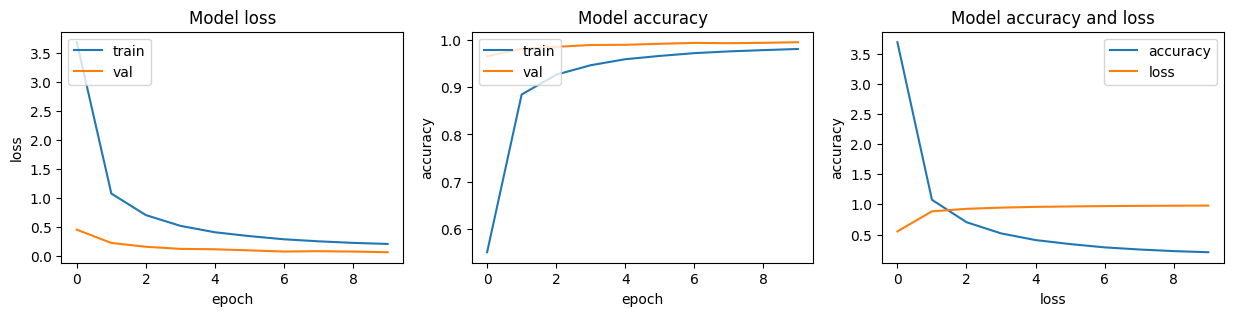
\includegraphics[width=\textwidth, height=\textheight,keepaspectratio]{task2/cnnModHyperLearningGraph}
    \caption[Learning graphs for hyperparameter tuned CNN with custom encoding]
    {Learning graphs for hyperparameter tuned CNN with custom encoding}
    \label{fig:cnnModHyperLearning}
\end{figure}

% \begin{figure}
%     \centering
%     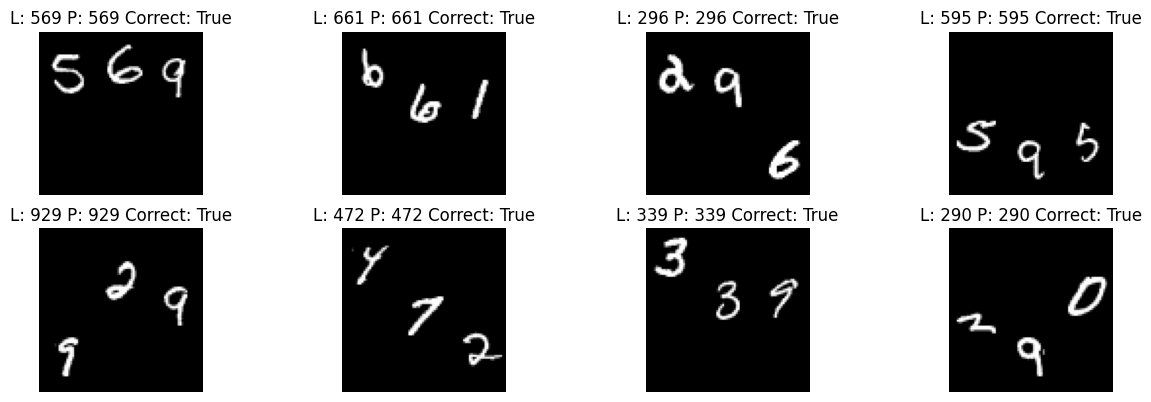
\includegraphics[width=\textwidth, height=\textheight,keepaspectratio]{task2/cnnModHyperPredictions}
%     \caption[Predictions for hyperparameter tuned CNN with custom encoding]
%     {Predictions for hyperparameter tuned CNN with custom encoding}
%     \label{fig:cnnModHyperPredictions}
% \end{figure}

\begin{figure}[!htbp]
    \centering
    \begin{subfigure}{0.3\textwidth}
        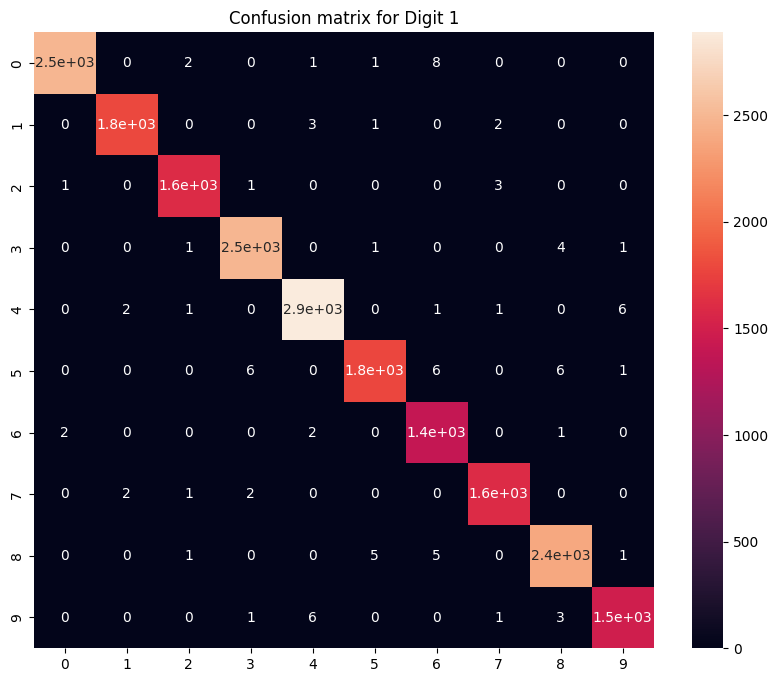
\includegraphics[width=\textwidth]{task2/cnnModHyperConfusion/digit1}
        \caption{Digit 1}
        \label{fig:cnnModHyperConfusionMatrix1}
    \end{subfigure}
    \begin{subfigure}{0.3\textwidth}
        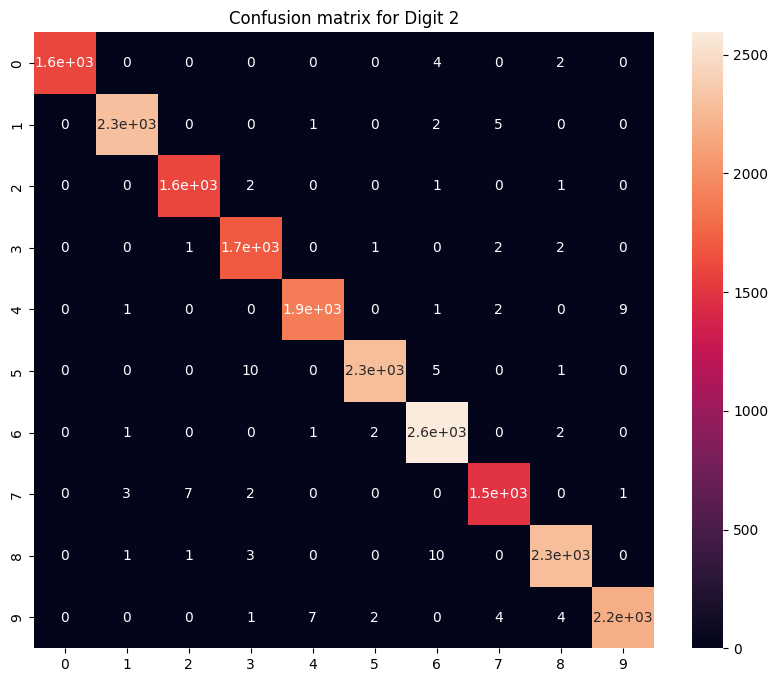
\includegraphics[width=\textwidth]{task2/cnnModHyperConfusion/digit2}
        \caption{Digit 2}
        \label{fig:cnnModHyperConfusionMatrix2}
    \end{subfigure}
    \begin{subfigure}{0.3\textwidth}
        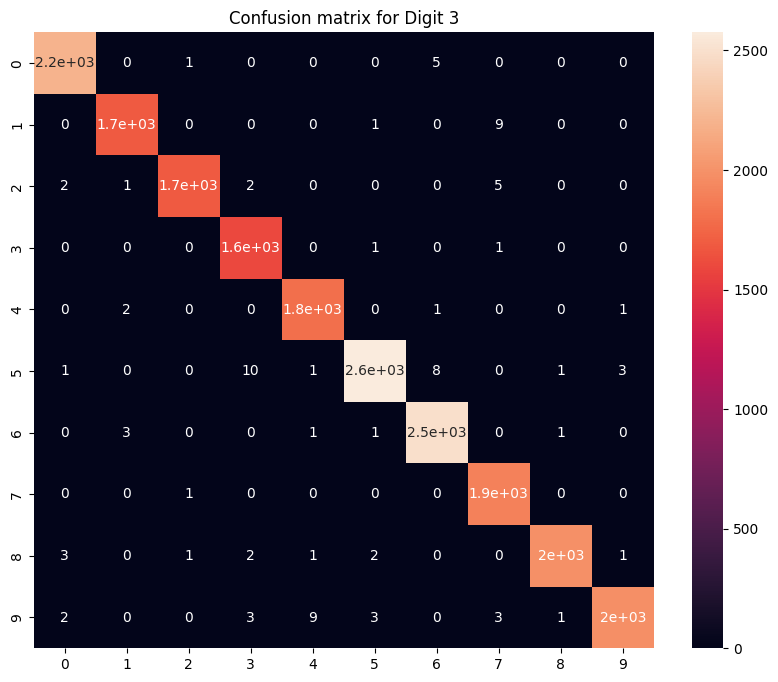
\includegraphics[width=\textwidth]{task2/cnnModHyperConfusion/digit3}
        \caption{Digit 3}
        \label{fig:cnnModHyperConfusionMatrix3}
    \end{subfigure}
    \caption{Confusion matrices for hyperparameter tuned CNN with custom encoding}
    \label{fig:cnnModHyperConfusionMatrix}
\end{figure}

\bgroup
    \begin{table}[!htbp]
        \centering
        \begin{tabular}{l|cc}
            \hline
            & Accuracy & F1 Score \\ \hline
            Digit 1 & 0.9954 & 0.9952 \\
            Digit 2 & 0.9948 & 0.9947 \\ 
            Digit 3 & 0.9953 & 0.9953 \\
        \end{tabular}
        \caption{Accuracy and F1 scores for hyperparameter tuned CNN with custom encoding}
        \label{tbl:accuracyCNNModHyper}
    \end{table}
\egroup

Despite this model performing an order of magnitude better than the previous CNN plus classifier without custom encoding, there are still improvements that can be made with the architecture of the network. Currently no learning from each digit location can be transferred. For instance, if the digit zero never appears in position one in the training set but is present in position two and three. When tested with a zero in position one the model will likely be unable to classify the digit. Ideally the classification task should be shared across each digit location, to produce a more robust classification model.

\pagebreak
\subsection{Decision Tree}
To collect another baseline performance metric, we shall use a simple decision tree model with no additional encoding techniques. Fitting a decision tree with varying depth levels should display if the model is overfitting when the train and test sets are compared.

\autoref{fig:decisionTreeLearning} displays the comparison between class and digit accuracies achieved, the model is initially underfitting then immediately overfitting. In contrast to the previous CNN the decision tree is unable to find the underlying patterns in the datasets. A per-digit accuracy of 18.72\% is achieved on the unseen test set, which is marginally above statistical chance (10\%), considerably worse than 66.56\%.

\begin{figure}[!htbp]
    \centering
    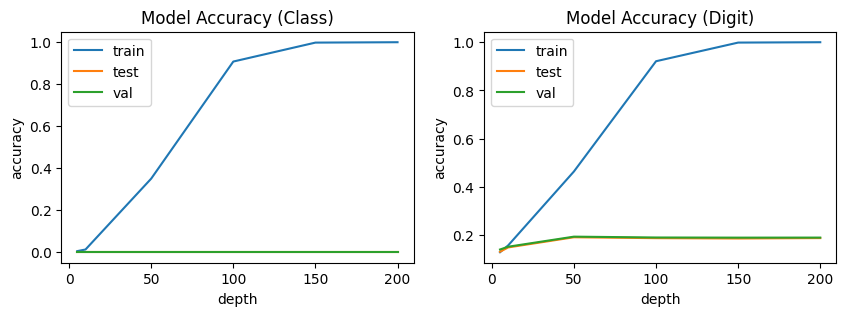
\includegraphics[width=\textwidth, height=5cm,keepaspectratio]{task2/decisionTreeLearningGraph}
    \caption[Learning graphs for decision tree]
    {Learning graphs for decision tree}
    \label{fig:decisionTreeLearning}
\end{figure}

% \begin{figure}
%     \centering
%     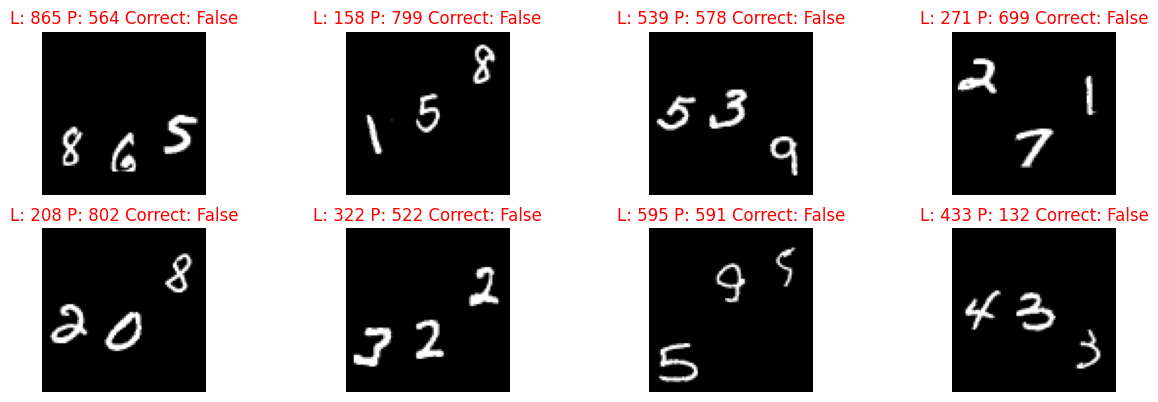
\includegraphics[width=\textwidth, height=5cm,keepaspectratio]{task2/decisionTreePredictions}
%     \caption[Predictions for decision tree]
%     {Predictions for decision tree}
%     \label{fig:decisionTreePredictions}
% \end{figure}

The decision tree appears to perform slightly better with the digit zero, this is likely a random pattern. Position one performs somewhat better in comparison to the other positions. Overall, the confusion matrices do show that the tree fails to classify most digits and the decision tree is a poor model.

\begin{figure}[!htbp]
    \centering
    \begin{subfigure}{0.3\textwidth}
        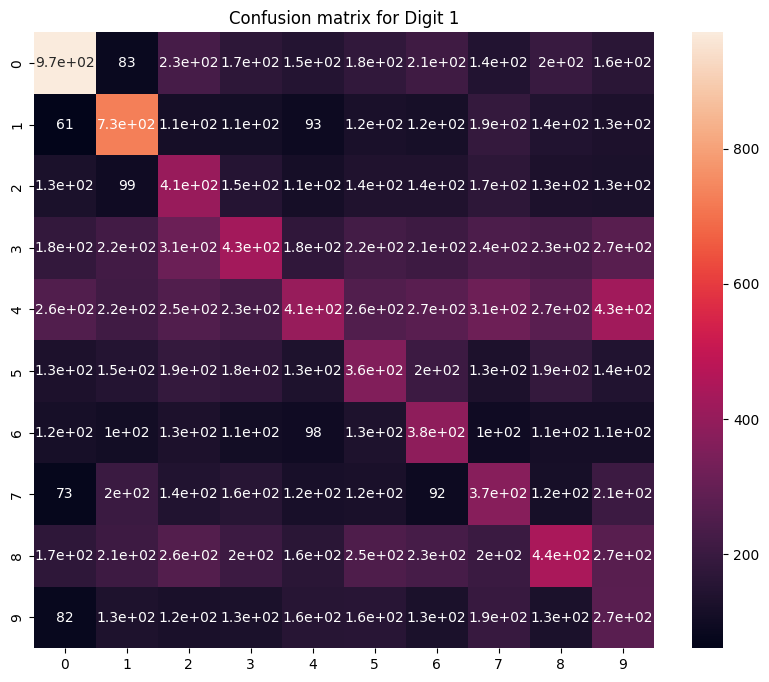
\includegraphics[width=\textwidth]{task2/decisionTreeConfusion/digit1}
        \caption{Digit 1}
        \label{fig:decisionTreeConfusionMatrix1}
    \end{subfigure}
    \begin{subfigure}{0.3\textwidth}
        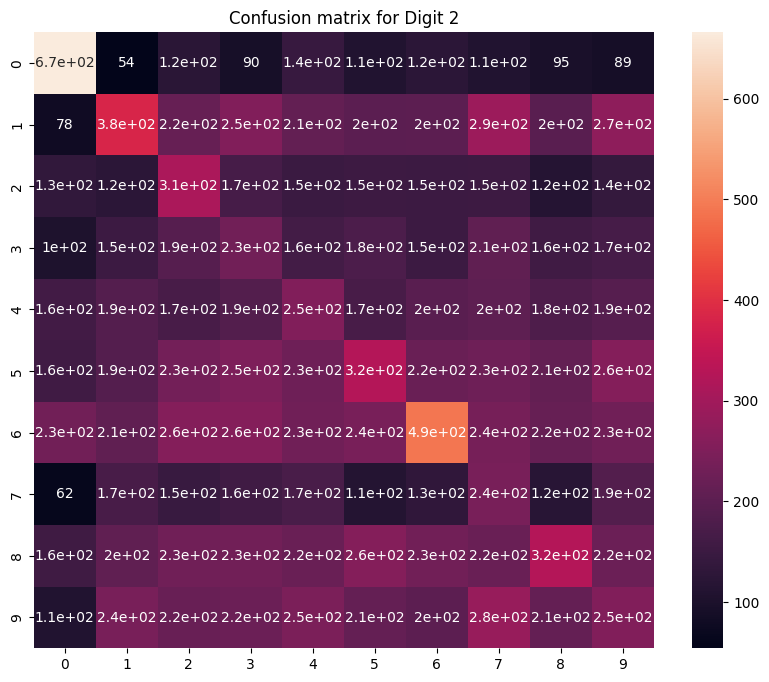
\includegraphics[width=\textwidth]{task2/decisionTreeConfusion/digit2}
        \caption{Digit 2}
        \label{fig:decisionTreeConfusionMatrix2}
    \end{subfigure}
    \begin{subfigure}{0.3\textwidth}
        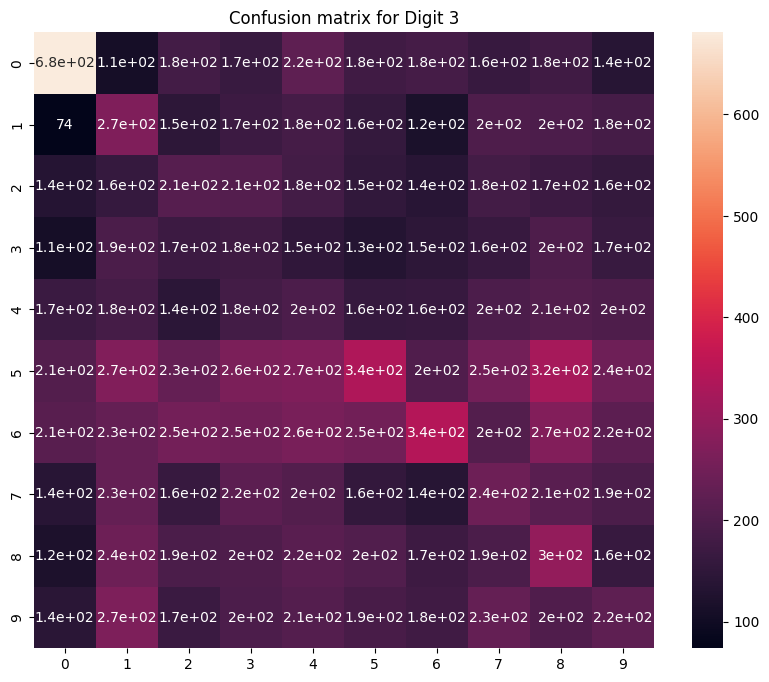
\includegraphics[width=\textwidth]{task2/decisionTreeConfusion/digit3}
        \caption{Digit 3}
        \label{fig:decisionTreeConfusionMatrix3}
    \end{subfigure}
    \caption{Confusion matrices for decision tree}
    \label{fig:decisionTreeConfusionMatrix}
\end{figure}

In an attempt to reduce overfitting, the model shall undergo tuning using Sklearn's GridSearchCV. This function performs cross-validation, so that the model is discouraged from learning the training set too well. While cross validation is taking place, hyperparameters shall be tuned using the values in in \autoref{tbl:hyperDecisionTree}. 

\bgroup
    \begin{table}[!htbp]
        \centering
        \begin{tabular}{ll|c}
            \hline
            Parameter & Values & Selected \\ \hline
            max\_depth & 5, 10, 50, 100, 150, 200 & 200 \\
        \end{tabular}
        \caption{Hyperparameter values for decision tree}
        \label{tbl:hyperDecisionTree}
    \end{table}

Due to the additional steps taken to reduce overfitting, the model is now underfitting. The decision tree is unable to capture the true pattern in the dataset. An overall accuracy of 18.96\% is achieved using the test set and is displayed in \autoref{fig:decisionTreeHyperLearning}. The confusion matrices in \autoref{fig:decisionTreeHyperConfusionMatrix} display a tendency for the model to predict the class one, this is likely a random pattern as the distribution of digits in the training set is even.

\begin{figure}[!htbp]
    \centering
    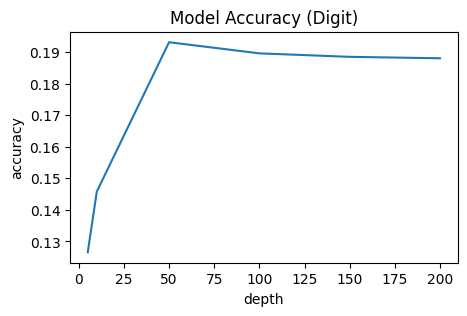
\includegraphics[width=\textwidth, height=5cm,keepaspectratio]{task2/decisionTreeHyperLearningGraph}
    \caption[Learning graphs for hyperparameter tuned decision tree]
    {Learning graphs for hyperparameter tuned decision tree}
    \label{fig:decisionTreeHyperLearning}
\end{figure}

% \begin{figure}
%     \centering
%     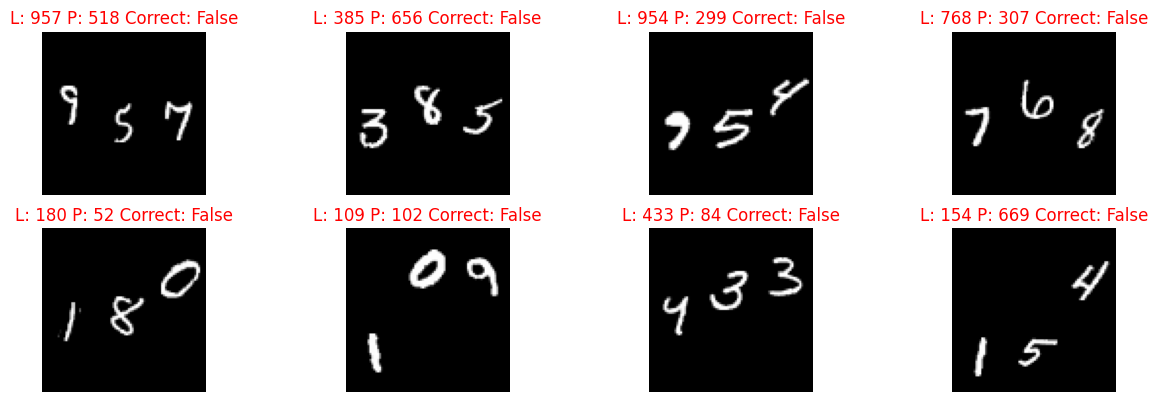
\includegraphics[width=\textwidth, height=5cm,keepaspectratio]{task2/decisionTreeHyperPredictions}
%     \caption[Predictions for hyperparameter tuned decision tree]
%     {Predictions for hyperparameter tuned decision tree}
%     \label{fig:decisionTreeHyperPredictions}
% \end{figure}

\begin{figure}[!htbp]
    \centering
    \begin{subfigure}{0.3\textwidth}
        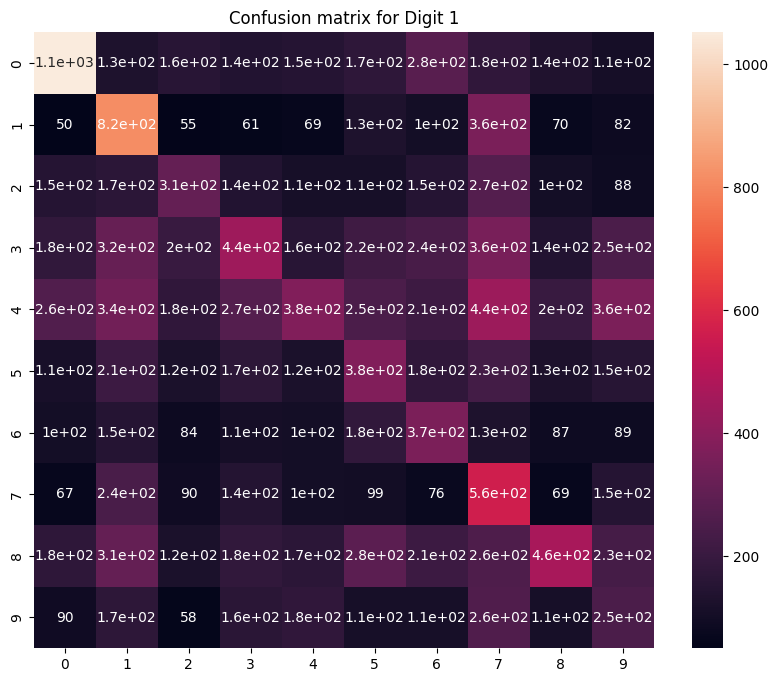
\includegraphics[width=\textwidth]{task2/decisionTreeHyperConfusion/digit1}
        \caption{Digit 1}
        \label{fig:decisionTreeHyperConfusionMatrix1}
    \end{subfigure}
    \begin{subfigure}{0.3\textwidth}
        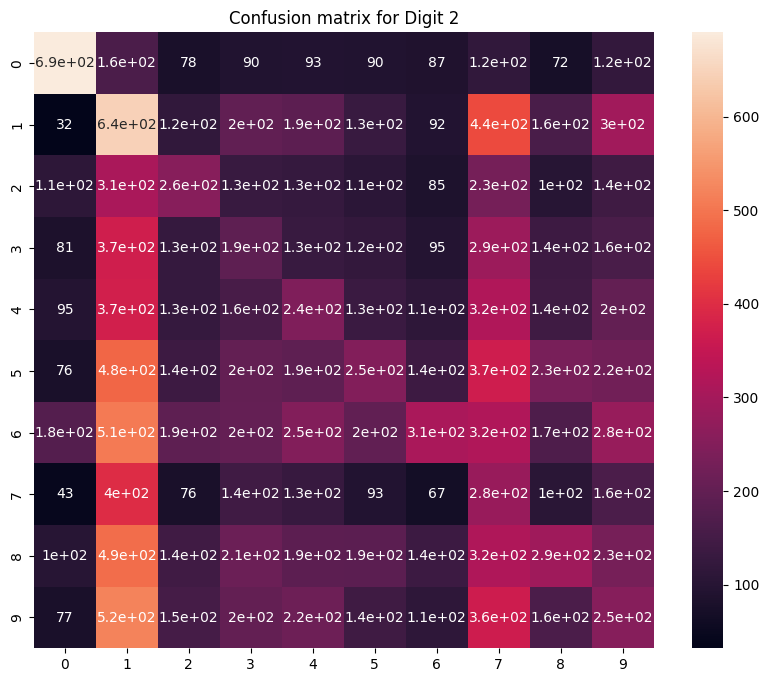
\includegraphics[width=\textwidth]{task2/decisionTreeHyperConfusion/digit2}
        \caption{Digit 2}
        \label{fig:decisionTreeHyperConfusionMatrix2}
    \end{subfigure}
    \begin{subfigure}{0.3\textwidth}
        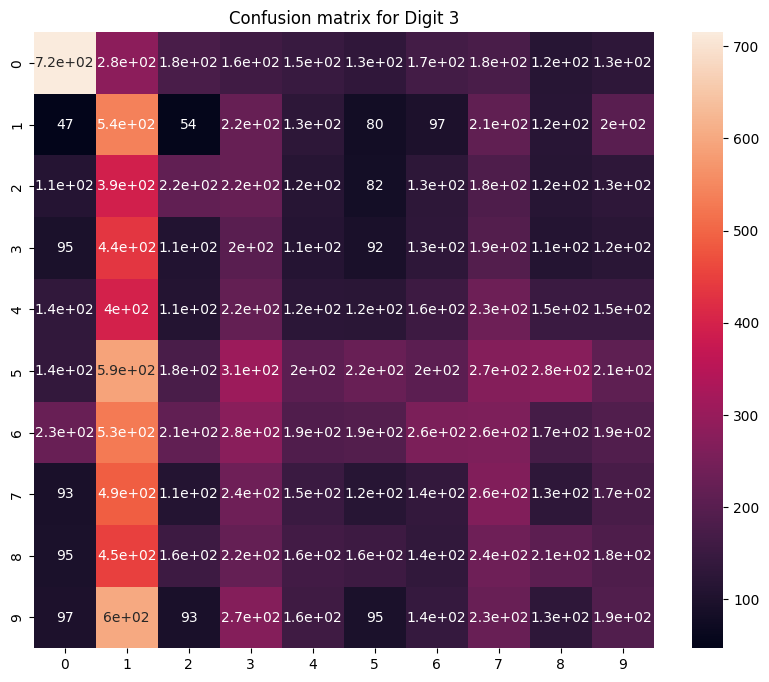
\includegraphics[width=\textwidth]{task2/decisionTreeHyperConfusion/digit3}
        \caption{Digit 3}
        \label{fig:decisionTreeHyperConfusionMatrix3}
    \end{subfigure}
    \caption{Confusion matrices for hyperparameter tuned decision tree}
    \label{fig:decisionTreeHyperConfusionMatrix}
\end{figure}

The decision trees have performed poorly in comparison to the CNN models because they do not contain methods to learn the hierarchical features within images. With increased depth and data, it could be possible for a decision tree to slowly learn these relationships.

\pagebreak
\section{Multi-Model Convolutional Neural Network}

To individually classify digits, the digits must be first split into separate images. There are several methods for splitting multiple digits (words) into individual digits (characters) for use with a classification model.

\subsection{Image Splitting}
A slice operation separates the image along pre-defined boundaries. This assumes that there are exactly three digits and that they are similarly placed across the data set. To reduce the individual character image size, the digits are also cropped horizontally with the presence of a digit in the top pixel row.

\begin{figure}[!htbp]
    \centering
    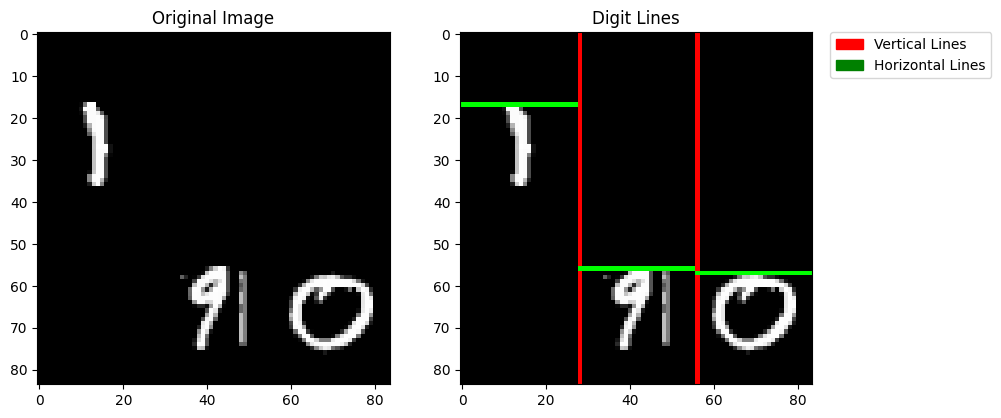
\includegraphics[width=\textwidth, height=4cm,keepaspectratio]{task3/simpleSplitProcess}
    \caption[Simple image splitting process]
    {Simple image splitting process}
    \label{fig:simpleSplitProcess}
\end{figure}

\begin{figure}[!htbp]
    \centering
    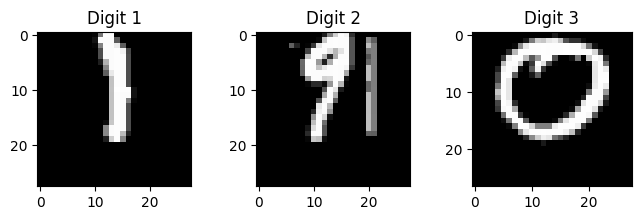
\includegraphics[width=\textwidth, height=2cm,keepaspectratio]{task3/simpleSplitResult}
    \caption[Simple image splitting result]
    {Simple image splitting result}
    \label{fig:simpleSplitResult}
\end{figure}

This method could work well in a pre-defined scenario. Though, it is likely to struggle in a real-world implementation where there could be any number of digits at random locations within the image.

\pagebreak
Another method dynamically divides the images using zero-filled columns and rows. When a column with every pixel value of zero is found, followed by a non-empty column, the image is cropped. The process is repeated in the horizontal dimension using rows.

\begin{figure}[!htbp]
    \centering
    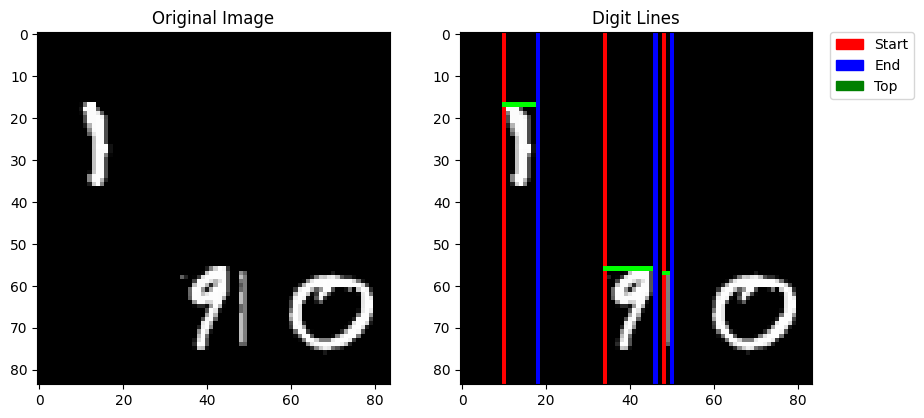
\includegraphics[width=\textwidth, height=4cm,keepaspectratio]{task3/dynamicSplitProcess}
    \caption[Dynamic image splitting process]
    {Dynamic image splitting process}
    \label{fig:dynamicSplitProcess}
\end{figure}

\begin{figure}[!htbp]
    \centering
    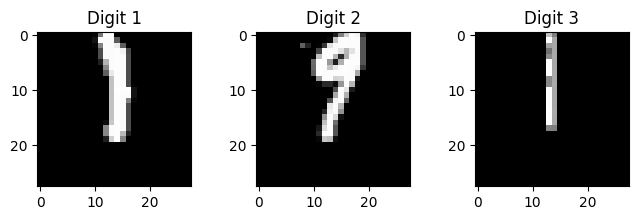
\includegraphics[width=\textwidth, height=2cm,keepaspectratio]{task3/dynamicSplitResult}
    \caption[Dynamic image splitting result]
    {Dynamic image splitting result}
    \label{fig:dynamicSplitResult}
\end{figure}

This relies on the assumption the digits do not overlap in either the horizontal or vertical dimensions. To prevent noise or digits with broken lines being accidently split supplementary checks are required. Examples of the splitting process failing are shown in the report's appendix, these could benefit from such checks.

\pagebreak
A more complex, but robust technique for separating the numbers into digits is using contour detection. 

The difference of white to black is used to generate continuous contours around a digit, marked with the green outline. The contours are filtered so that objects with a very small area (14px) are removed. This should remove noise, such as pen smudges. Using the contours, a series of bounding boxes are created, marking where the images should be cropped. The cropped images are subsequently padded so that they fill a 28x28 image.

\begin{figure}[!htbp]
    \centering
    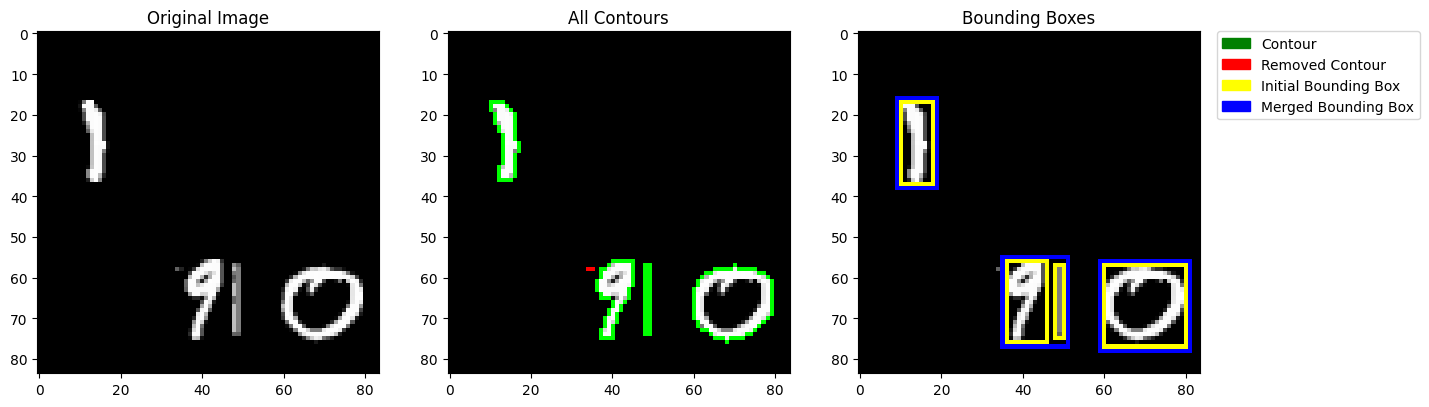
\includegraphics[width=\textwidth, height=4cm,keepaspectratio]{task3/contourSplitProcess}
    \caption[Contour image splitting process]
    {Contour image splitting process}
    \label{fig:contourSplitProcess}
\end{figure}

\begin{figure}[!htbp]
    \centering
    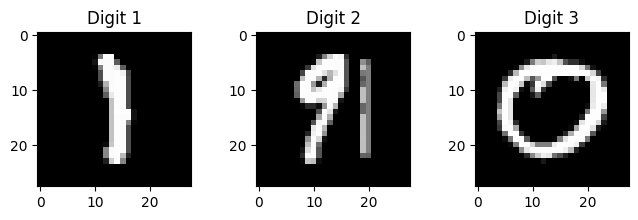
\includegraphics[width=\textwidth, height=2cm,keepaspectratio]{task3/contourSplitResult}
    \caption[Contour image splitting result]
    {Contour image splitting result}
    \label{fig:contourSplitResult}
\end{figure}

This method works well, until a digit has a break in its line. To combat this, we can merge cropped images together if they meet a specified threshold. If all digits are assumed to be 28x28, every contour merge pair can be tested. If the merge is wider or taller than 28px, the contours are not merged. The specific thresholds can be fine-tuned using hyperparameter tuning.

For this technique of splitting to be effective, the handwriting must not be cursive. This is unlikely to be the case with digits but there is still the possibility of digits touching. In this scenario, the contours of two digits would unintentionally join.

\pagebreak
\subsection{Convolutional Neural Network}

Although more complicated, integrating the image splitting directly into TensorFlow allows for hyperparameter tuning of the splitting layer itself. The optimum pair of splitter and classifier can be tuned together, rather than apart.

Multiple instances of the same base model are concatenated together into one larger model with the custom Keras splitting layer. Each base model takes one processed image from the splitting layer and performs classification. The output from each model is then concatenated back together. The same custom loss and accuracy functions are required from the previous CNN model. \autoref{fig:multiModelArchitecture} displays these repeated models using the dashed box border.

\begin{figure}[!htbp]
    \centering
    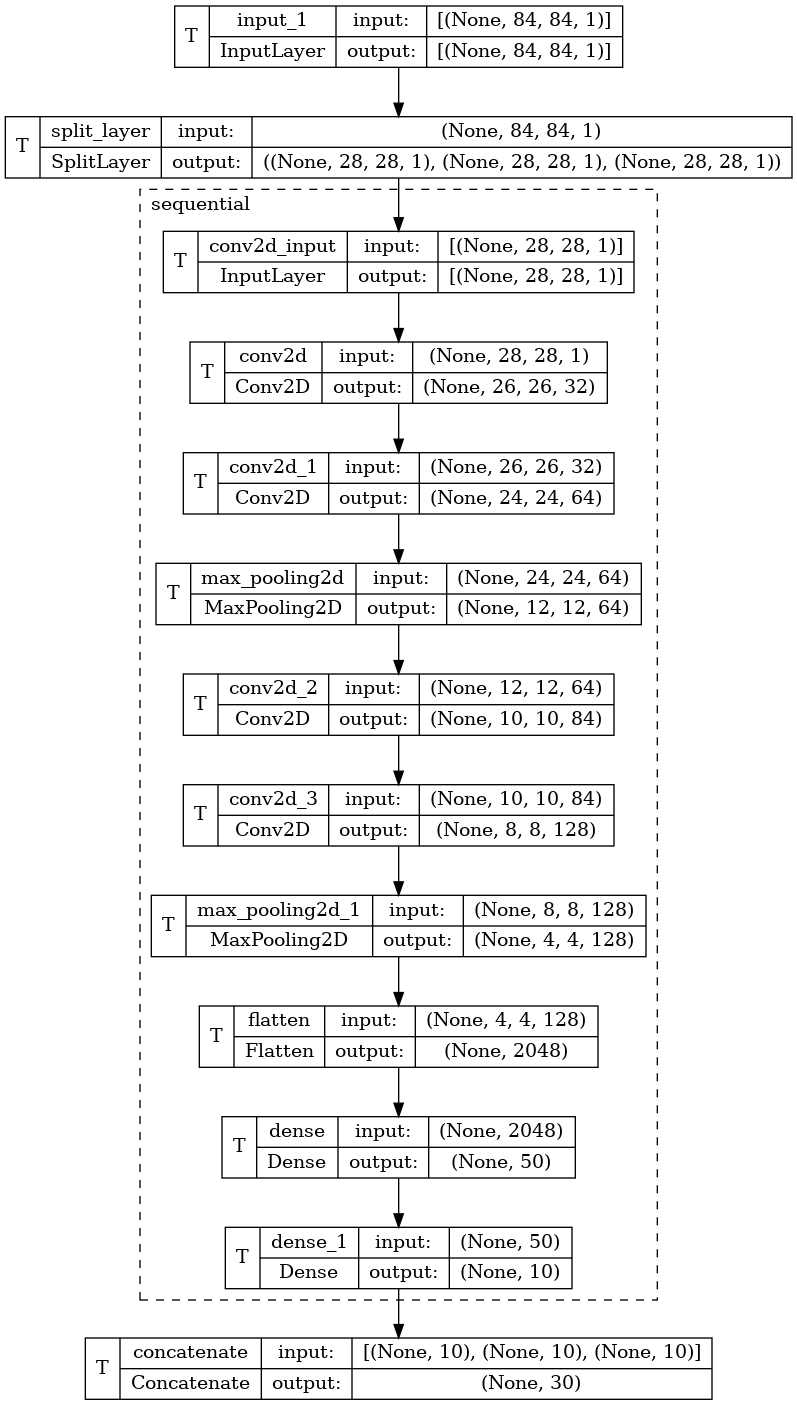
\includegraphics[width=\textwidth, height=16cm,keepaspectratio]{task2/multiModelArchitecture}
    \caption[Multi-model architecture]
    {Multi-model architecture}
    \label{fig:multiModelArchitecture}
\end{figure}

Note that the dropout layers are removed in this splitting CNN model, this is because the model struggled to train with them present. With additional epochs and tuning it is likely they could work so during hyperparameter tuning they shall be re-introduced. Although very slow to train this model performs with an overall accuracy of 99.58\%. The slow training is because the digit splitting layer is processed on the CPU, rather than GPU. The performance of this model could be improved if the splitting step was parallelised. No overfitting is apparent in \autoref{fig:cnnMultiLearning} and the model's performance is comparable to the single digit classifier from \autocite{biswasEfficientCNNModel2021}. However, despite the extra complexity, the model is marginally better than the CNN with a custom encoding method.

\begin{figure}[!htbp]
    \centering
    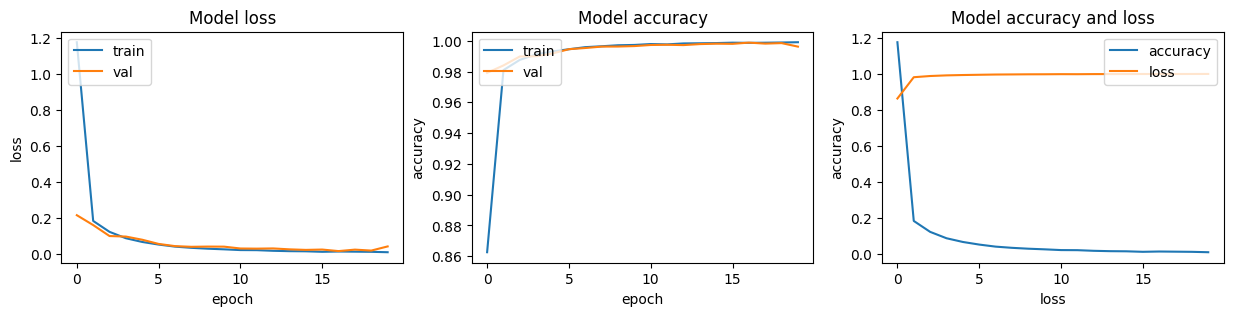
\includegraphics[width=\textwidth, height=\textheight,keepaspectratio]{task3/cnnMultiLearningGraph}
    \caption[Learning graphs for multi-model CNN]
    {Learning graphs for multi-model CNN}
    \label{fig:cnnMultiLearning}
\end{figure}

The values used for hyperparameter tuning are shown in \autoref{tbl:hyperCNNMulti}. Additional parameters for the splitting layer include contour size and threshold boundaries.

\bgroup
    \begin{table}[!htbp]
        \centering
        \begin{tabular}{ll|c}
            \hline
            Parameter & Values & Selected \\ \hline
            kernel\_size\_1 & 2, 3, 4, 5 & 4 \\
            kernel\_size\_2 & 2, 3, 4, 5 & 3 \\
            kernel\_size\_3 & 2, 3, 4, 5 & 3 \\
            kernel\_size\_4 & 2, 3, 4, 5 & 4 \\
            pool\_size\_1 & 2, 3, 4 & 2 \\
            pool\_siz\_2 & 2, 3, 4 & 2 \\
            dropout\_1 & 0.2, 0.8, step=0.1 & 0.4 \\
            dropout\_2 & 0.2, 0.8, step=0.1 & 0.2 \\
            dense\_layer\_units & 10, 50, 100 & 10 \\
            contour\_size & 0.001, 0.01, step=0.001 & 0.001 \\
            threshold\_lower & 0, 120, step=20 & 80 \\
            threshold\_upper & 135, 255, step=20 & 175 \\
            learning\_rate & min=0.0001, max=0.1, sampling="LOG" & 0.00021 \\
        \end{tabular}
        \caption{Hyperparameter values for multi-model CNN}
        \label{tbl:hyperCNNMulti}
    \end{table}
\egroup

Using the optimal parameters, a per-digit accuracy of 99.65\% is achieved on the test set with fifty epochs of training. The learning graphs in \autoref{fig:cnnMultiHyperLearning} display that the parameters found produce a slower training curve for the train set. This could be because the regularisation dropout layers are strong. Training for additional epochs could improve this score.

\begin{figure}[!htbp]
    \centering
    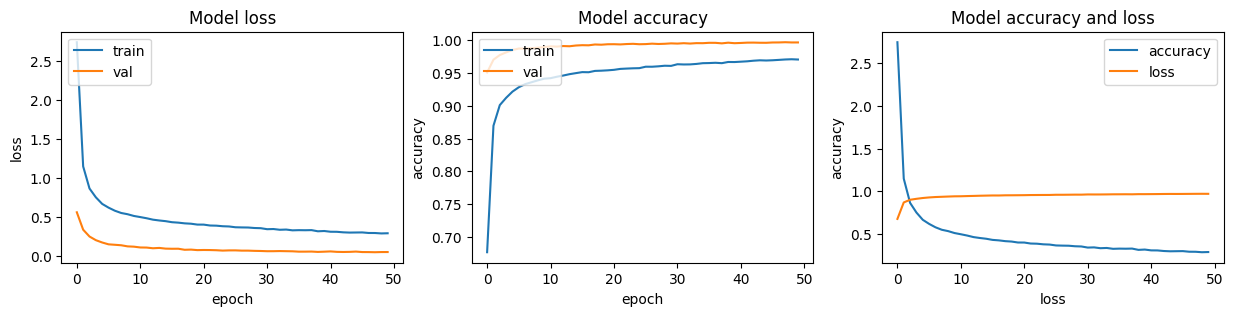
\includegraphics[width=\textwidth, height=\textheight,keepaspectratio]{task3/cnnMultiHyperLearningGraph}
    \caption[Learning graphs for hyperparameter tuned multi-model CNN]
    {Learning graphs for hyperparameter tuned multi-model CNN}
    \label{fig:cnnMultiHyperLearning}
\end{figure}

The final model performs excellently, with even digit distribution displayed in both \autoref{fig:cnnMultiHyperConfusionMatrix} and \autoref{tbl:accuracyCNNModHyper}. The heatmaps from the confusion matrices closely resemble the digit distribution heatmaps from initial visualisation.

\begin{figure}[!htbp]
    \centering
    \begin{subfigure}{0.3\textwidth}
        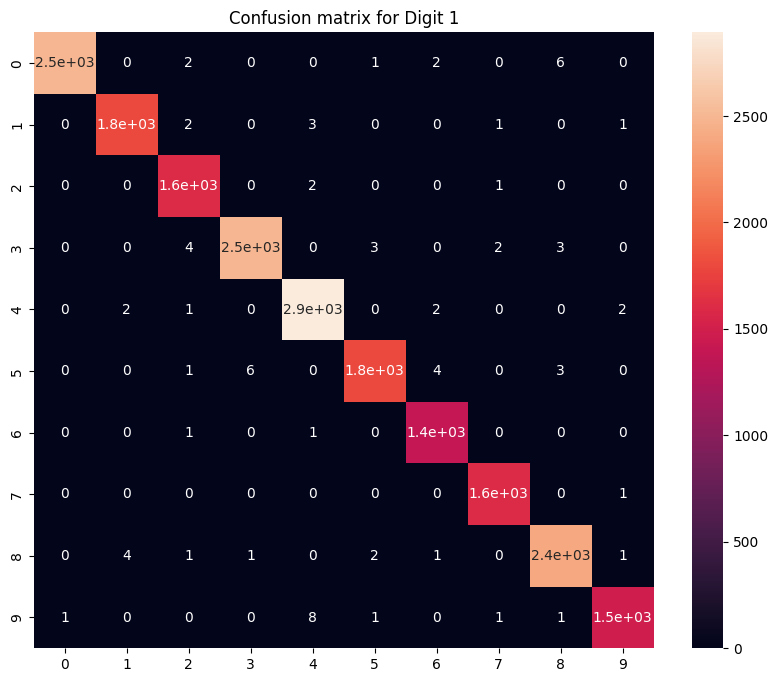
\includegraphics[width=\textwidth]{task3/cnnMultiHyperConfusion/digit1}
        \caption{Digit 1}
        \label{fig:cnnMultiHyperConfusionMatrix1}
    \end{subfigure}
    \begin{subfigure}{0.3\textwidth}
        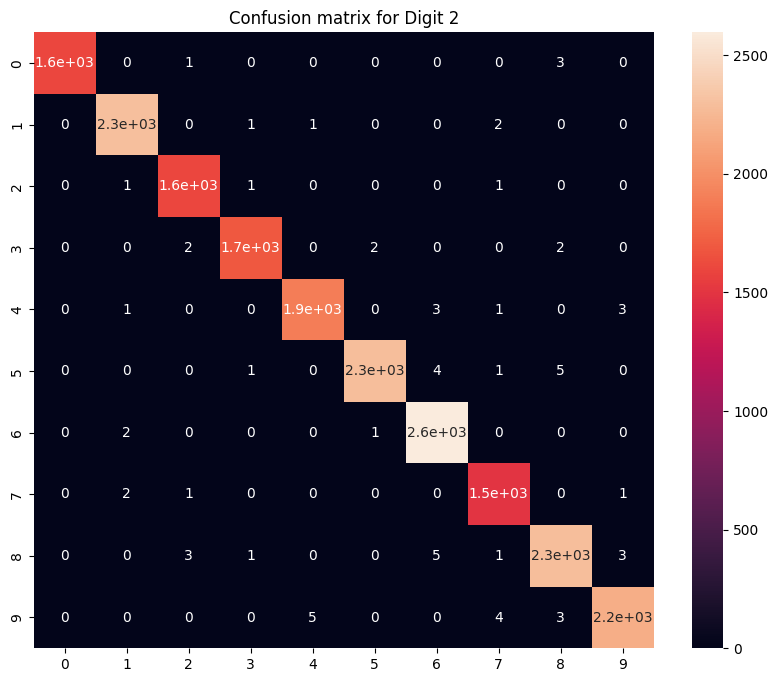
\includegraphics[width=\textwidth]{task3/cnnMultiHyperConfusion/digit2}
        \caption{Digit 2}
        \label{fig:cnnMultiHyperConfusionMatrix2}
    \end{subfigure}
    \begin{subfigure}{0.3\textwidth}
        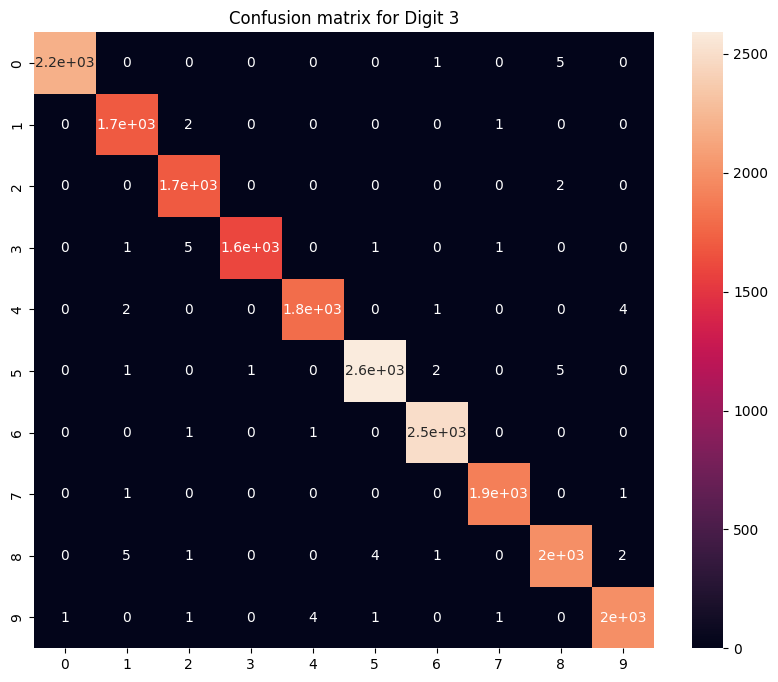
\includegraphics[width=\textwidth]{task3/cnnMultiHyperConfusion/digit3}
        \caption{Digit 3}
        \label{fig:cnnMultiHyperConfusionMatrix3}
    \end{subfigure}
    \caption{Confusion matrices for hyperparameter tuned multi-model CNN}
    \label{fig:cnnMultiHyperConfusionMatrix}
\end{figure}

\bgroup
    \begin{table}[!htbp]
        \centering
        \begin{tabular}{l|cc}
            \hline
            & Accuracy & F1 Score \\ \hline
            Digit 1 & 0.99605 & 0.99597836 \\
            Digit 2 & 0.9966 & 0.9966265 \\
            Digit 3 & 0.997 & 0.9969314 \\        
        \end{tabular}
        \caption{Accuracy and F1 scores for hyperparameter tuned multi-model CNN}
        \label{tbl:accuracyCNNMultiHyper}
    \end{table}
\egroup

The improved performance from this CNN model and splitting layer is realised because the single classifier is able to gain experience from every digit location. In a direct comparison to the simple CNN with encoding, the classification layers are trained on triple the amount of data. This reenforces the model’s learning of handwritten digits.

\pagebreak
\section{Optimisation}

The models developed all use advanced techniques to produce the most optimal multi-digit classifier. One of the best single MNIST classifiers achieves an accuracy of 99.87\% using homogeneous vector capsules \autocite{byerlyNoRoutingNeeded2021}. We could attempt to increase the current model's performance or build a new model for additional tasks.

One possible method to build a more generic handwriting recognition model is to use a recurrent neural network (RNN) \autocite{advaithHandwritingRecognitionUsing2021}. Typically, when classifying text there is a semantic relationship between each letter, this can aid the classification process by suggesting what characters are likely. An RNN can store this sequential relationship between letters. This kind of model would be unnecessary and impractical for a simple multi-digit classification problem as there is little relationship between each digit in an image. 

Another improvement technique could be to use an object recognition model to find text to classify within an image. This would involve taking a pre-trained model such as "ssd\_mobilenet\_v2" from TensorFlow and fine-tuning it on the handwritten digit dataset. However, object classification models are very large and are generally designed for much more complex image classification tasks.

Instead, to build a more diverse digit classification model, and hence more accurate, we will use data augmentation techniques. The CNN with custom encoding lacked exposure from every digit in comparison to the CNN with image splitting. The digits can be randomly rearranged so that every digit classifier can gain even experience from every digit, \autoref{fig:digitAugmentation}. This can be implemented within the dataset loading layer.

\begin{figure}[!htbp]
    \centering
    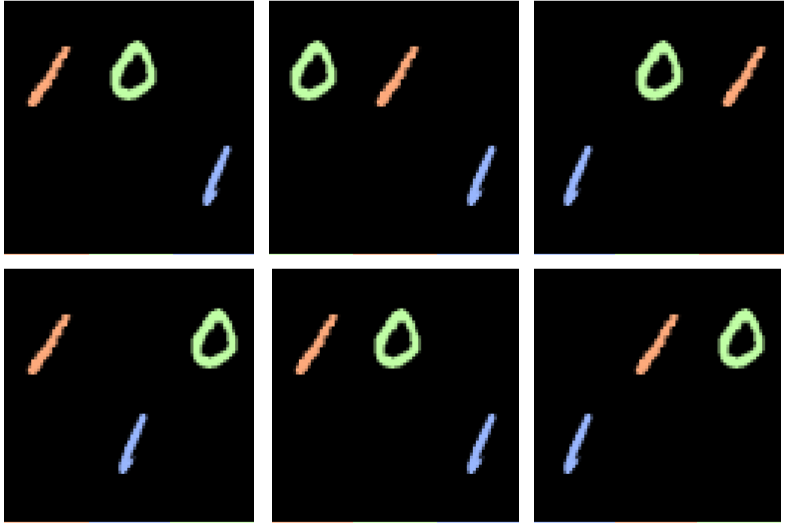
\includegraphics[width=\textwidth, height=4cm,keepaspectratio]{task4/digitAugmentation.png}
    \caption[Digit augmentation example]
    {Digit augmentation example}
    \label{fig:digitAugmentation}
\end{figure}

\pagebreak
In addition to the augmentation, the hyperparameter search can be expanded to find optimum layer sizes for the convolutional and pooling layers. This could significantly increase the tuning time but increase the model's performance.

\bgroup
    \begin{table}[!htbp]
        \centering
        \begin{tabular}{ll|c}
            \hline
            Parameter & Values & Selected \\ \hline
            kernel\_size\_1 & 2, 3, 4, 5 & 3 \\
            kernel\_size\_2 & 2, 3, 4, 5 & 5 \\
            kernel\_size\_3 & 2, 3, 4, 5 & 4 \\
            kernel\_size\_4 & 2, 3, 4, 5 & 5 \\
            pool\_size\_1 & 2, 3, 4 & 4 \\
            pool\_size\_2 & 2, 3, 4 & 4 \\
            conv2d\_1 & min=32, max=256, step=32 & 32 \\
            conv2d\_2 & min=32, max=256, step=32 & 128 \\
            conv2d\_3 & min=32, max=256, step=32 & 256 \\
            conv2d\_4 & min=32, max=256, step=32 & 32 \\
            dropout\_1 & 0.2, 0.8, step=0.1 & 0.5 \\
            dense\_layer\_units & 64, 128, 256, 512, 1024 & 64 \\
            learning\_rate & min=0.0001, max=0.1, sampling="LOG" & 0.00014 \\
        \end{tabular}
        \caption{Hyperparameter values for CNN with custom encoding and augmentation}
        \label{tbl:hyperCNNModAug}
    \end{table}
\egroup

A final accuracy of 99.91\% is observed on the test set, using the tuned hyperparameters, after one hundred epochs of training. Despite the increased model complexity and training time, the model is not overfitting and performs well on the unseen data, \autoref{fig:cnnModAugHyperLearning}.

\begin{figure}[!htbp]
    \centering
    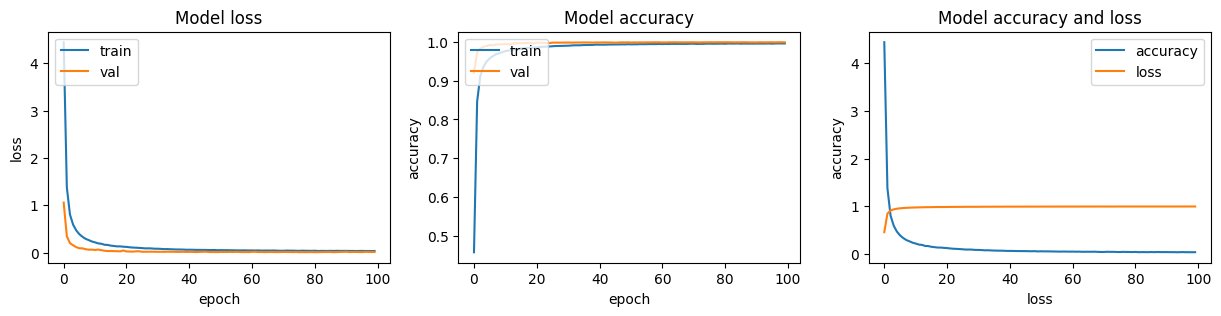
\includegraphics[width=\textwidth, height=\textheight,keepaspectratio]{task4/cnnModAugHyperLearningGraph}
    \caption[Learning graphs for hyperparameter tuned CNN with custom encoding and augmentation]
    {Learning graphs for hyperparameter tuned CNN with custom encoding and augmentation}
    \label{fig:cnnModAugHyperLearning}
\end{figure}

The diagram in \autoref{fig:cnnAltArchitecture} displays the slight modifications made to the combined CNN architecture. The digit classification head layers were separated, this provides no performance benefit but clarifies the model's behaviour. The image includes the tuned hyperparameter values for each layer size.

\begin{figure}[!htbp]
    \centering
    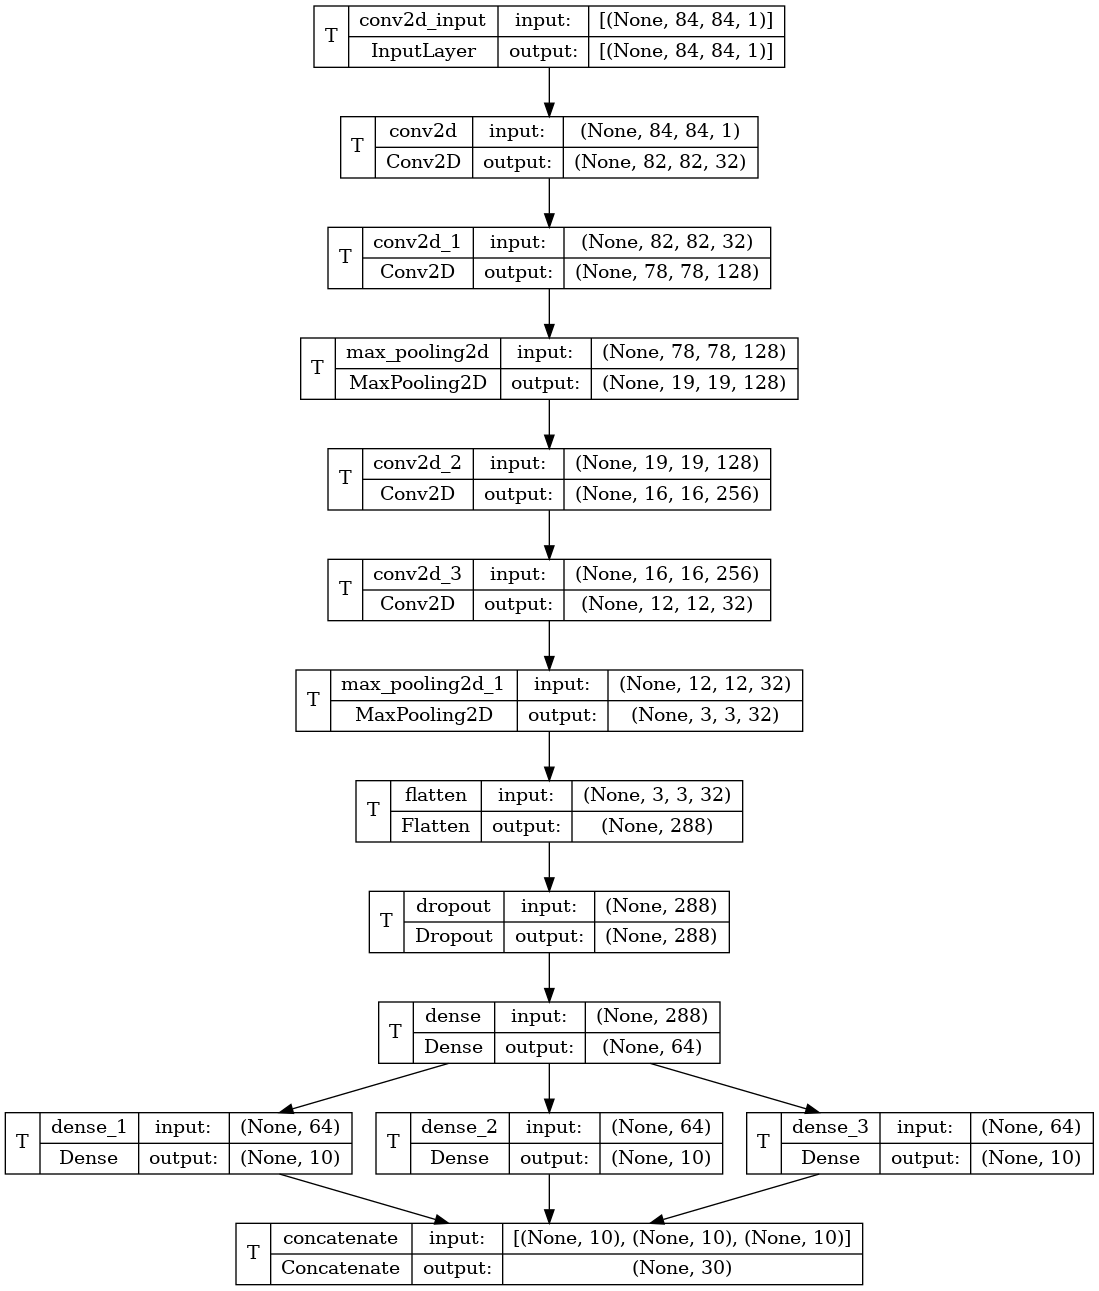
\includegraphics[width=\textwidth, height=16cm,keepaspectratio]{task4/cnnAltArchitecture}
    \caption[Modified multi-head CNN architecture]
    {Modified multi-head CNN architecture}
    \label{fig:cnnAltArchitecture}
\end{figure}

\begin{figure}[!htbp]
    \centering
    \begin{subfigure}{0.3\textwidth}
        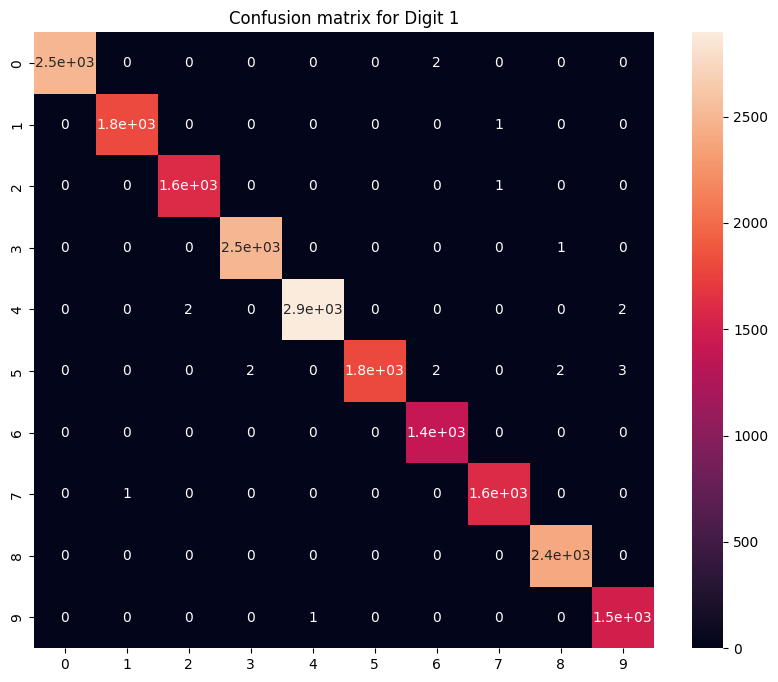
\includegraphics[width=\textwidth]{task4/cnnModAugHyperConfusion/digit1}
        \caption{Digit 1}
        \label{fig:cnnModAugHyperConfusionMatrix1}
    \end{subfigure}
    \begin{subfigure}{0.3\textwidth}
        \includegraphics[width=\textwidth]{task4/cnnModAugHyperConfusion/digit2}
        \caption{Digit 2}
        \label{fig:cnnModAugHyperConfusionMatrix2}
    \end{subfigure}
    \begin{subfigure}{0.3\textwidth}
        \includegraphics[width=\textwidth]{task4/cnnModAugHyperConfusion/digit3}
        \caption{Digit 3}
        \label{fig:cnnModAugHyperConfusionMatrix3}
    \end{subfigure}
    \caption{Confusion matrices for hyperparameter tuned CNN with custom encoding and augmentation}
    \label{fig:cnnModAugHyperConfusionMatrix}
\end{figure}
\chapter{Conclusion}
Several machine learning techniques have been applied to a multi-digit classification problem. We reduced the classification space from one thousand to thirty by encoding the model using multi-label methods. The simple CNN models dramatically outperformed the decision tree models due to them being better suited to hierarchical feature learning. 

Next, we tested splitting the images with a variety of techniques and performing classification on single digits at a time. This yields a small but significant increase in performance. The final model does not use a splitting layer, this allows the entire model to be trained on a GPU which is much faster. Because of the increased performance, more in-depth hyperparameter tuning could take place. An accuracy of 99.93\% is achieved. The majority of the failed classifications would be exceptionally challenging for a human to interpret also. In some cases, the provided labels in the dataset could be considered incorrect, examples are shown in \autoref{tbl:accuracyComparison}.

\vspace{10pt}
\bgroup
    \begin{table}[!htbp]
        \centering
        \begin{tabular}{ccccc}
            \hline
            Simple CNN & Simple CNN (encoding) & Decision Tree & Splitting CNN & Final CNN \\ \hline
            66.56\% & 99.51\% & 18.96\% & 99.65\% & 99.93\% \\
        \end{tabular}
        \caption{Accuracy of models}
        \label{tbl:accuracyComparison}
    \end{table}
\egroup




% ----------------------
% |    Bibliography    |
% ----------------------
\printbibliography

\end{document}
